% !TEX TS-program = pdflatexmk
% ================================================================
%  Bachelor's Thesis Template
%  Font: Times New Roman (newtxtext + newtxmath)
%  Line spacing: 1.5
%  Margins: top/bottom/right 3cm, left 3.5cm (binding)
%  Bibliography: author-year (biber) — use \citet and \citep
% ================================================================

\documentclass[12pt, a4paper, oneside]{report}

% ── Encoding & Language ─────────────────────────────────────
\usepackage[T1]{fontenc}
\usepackage[utf8]{inputenc}
\usepackage[english]{babel}

% ── Times New Roman (text + math) ───────────────────────────
\usepackage{mathptmx}   % Times New Roman text + math

% ── Page Layout ─────────────────────────────────────────────
\usepackage[
  top    = 3cm,
  bottom = 3cm,
  left   = 3.5cm,        % extra space for binding
  right  = 3cm
]{geometry}

% ── Line Spacing ────────────────────────────────────────────
\usepackage{setspace}
\onehalfspacing

% ── Math ────────────────────────────────────────────────────
\usepackage{amsmath}
\usepackage{amssymb}
\numberwithin{equation}{section}
\usepackage{amsthm}

% ── Tables ──────────────────────────────────────────────────
\usepackage{booktabs}
\usepackage{array}
\usepackage{siunitx}
\usepackage{caption}
% Improved tables
\usepackage{tabularx}
\usepackage{longtable}

% ── Graphics & Plots ────────────────────────────────────────
\usepackage{graphicx}
\usepackage{pgfplots}
\pgfplotsset{compat=1.18}
\usepackage{float}
\usepackage{subfigure}


% Improved verbatim appearance
\usepackage{fancyvrb}


% ── Colours ─────────────────────────────────────────────────
\usepackage{xcolor}
\definecolor{navyblue}{RGB}{0, 44, 95}

% ── Bibliography: author-year ───────────────────────────────
%    In the text use:
%      \citet{key}   →  Author (Year)
%      \citep{key}   →  (Author, Year)
%      \citep[p.~5]{key}  →  (Author, Year, p. 5)
%\usepackage[authoryear, round, sort]{natbib}
%\bibliographystyle{apalike}

\usepackage[style=authoryear, backend=biber]{biblatex}
\addbibresource{bib/Bibliography.bib}
%\let\cite\parencite
\let\citep\parencite
\let\cite\textcite

% ── Hyperlinks ──────────────────────────────────────────────
\usepackage[
  colorlinks = true,
  linkcolor  = navyblue,
  citecolor  = navyblue,
  urlcolor   = navyblue
]{hyperref}

% ── Chapter Style ───────────────────────────────────────────
\usepackage{titlesec}
\titleformat{\chapter}[display]
  {\normalfont\huge\bfseries}
  {\chaptertitlename\ \thechapter}
  {14pt}{\Huge}
\titlespacing*{\chapter}{0pt}{30pt}{20pt}

% ── Header / Footer ─────────────────────────────────────────
\usepackage{fancyhdr}
\pagestyle{fancy}
\fancyhf{}
\fancyhead[L]{\small\nouppercase{\leftmark}}
\fancyhead[R]{\small\thepage}
\renewcommand{\headrulewidth}{0.4pt}

% ── Theorem Environments ────────────────────────────────────
\newtheorem{theorem}{Theorem}[chapter]
\newtheorem{definition}[theorem]{Definition}

% ── Filler text (remove in the real thesis) ─────────────────
\usepackage{lipsum}

% ================================================================
%  THESIS METADATA  — fill in your details
% ================================================================
\newcommand{\thesistitle}{Title of the Bachelor's Thesis}
\newcommand{\thesissubtitle}{An Optional Subtitle}
\newcommand{\authorname}{First Name Last Name}
\newcommand{\studentid}{Student ID: 000000}
\newcommand{\supervisor}{Prof.\ Jane Doe}
\newcommand{\cosupervisor}{Dr.\ John Smith}   % delete if not applicable
\newcommand{\department}{Department of \ldots}
\newcommand{\university}{University Name}
\newcommand{\programme}{Bachelor's Degree in \ldots}
\newcommand{\academicyear}{Academic Year 2025/2026}

% ================================================================
\begin{document}
% ---------------------------------------------
% COVER PAGE (frontespizio) - fragment to \input
% Requires in the main preamble:
%   \usepackage{graphicx}
%   \usepackage{ragged2e}
% and units_logo.png in the same folder / graphics path
% ---------------------------------------------
\begin{titlepage}
\pagestyle{empty}
\begin{center}

% --- Logo ---

\includegraphics[width=3.2cm]{img/units_logo.png}

\vspace{0.6em}
\rule{0.85\textwidth}{0.4pt}
\vspace{1.2em}

% --- Department / Programme / Type ---
{\large\bfseries Department of Economics, Business, Mathematics and Statistics \par}
\vspace{1.5em}
{\large\bfseries Degree Programme in \\ Business Administration and Management \par}
\vspace{0.4em}
{\large\bfseries Curriculum: Business and Management \par}
\vspace{3.5em}
{\large\bfseries BACHELOR'S THESIS \par}

\vspace{0.4em}

% --- Title ---
{\Large\bfseries Economic, Social, and Pandemic Determinants of Video Game Sales: A Cross-National Analysis Using Mixed-Effects Models  \par}

\end{center}

\vfill

% --- Candidate / Supervisor ---
{\large
    \setlength{\tabcolsep}{12pt}

    \begin{tabularx}{\linewidth}{ >{\raggedleft}X >{\raggedright\arraybackslash}X}
        Candidate & Supervisor \\
        \bfseries Roberto Maijnelli & \bfseries Prof. Gioia Di Credico \\ [5mm]
    \end{tabularx}
}

\vspace{2em}

\begin{center}
{\bfseries ACADEMIC YEAR 2025 -- 2026}
\end{center}

\end{titlepage} 
\clearpage

% ── Dedication Page ─────────────────────────────────────────────
\newpage
\thispagestyle{empty}
\vspace*{5cm}
\begin{flushright}
  \itshape
  To my family and friends,\\
  who supported me throughout this journey.
\end{flushright}
\clearpage

% ── Front Matter (roman page numbers) ───────────────────────────
\pagenumbering{roman}
\setcounter{page}{1}

% Abstract ───────────────────────────────────────────────────────
\chapter*{Abstract}

This thesis analyzes the evolution of video game industry 
revenues over the period 2014–2024, with the objective of 
identifying the main macroeconomic, social, and pandemic-related
determinants of sales across a sample of 39 countries.\\
The analysis combines an exploratory descriptive investigation 
with a Generalized Additive Model with random intercepts (GAM + re), which accounts 
for regional heterogeneity across countries and allows for the 
estimation of non-linear relationships between the predictors 
and the response variable.\\
The model includes GNI per capita, internet penetration, 
unemployment rate, and a tensor product smooth interaction 
between year and depression rates, alongside a continent-level 
random effect. The results indicate that purchasing power follows 
a linear trend, while internet penetration, unemployment, and the 
temporal evolution of depression rates operate through complex 
non-linear paths. Geographic heterogeneity across continents 
accounts for a substantial share of the variance in sales.\\
A notable limitation concerns the Stringency Index, which proved to be
non-significant in the final model despite descriptive evidence 
suggesting a short-term spike in sales during the initial COVID-19 
lockdowns. This discrepancy is attributed to the temporal 
aggregation of the index across a three-year period, which likely 
smoothed out the short-term behavioral response.\\
Overall, the findings suggest that structural and psychological 
factors are more persistent determinants of video game demand than 
short-term pandemic shocks, contributing to a broader macroeconomic 
understanding of the global entertainment industry.
This study contributes to the existing literature by investigating
some of the plausible drivers of video game sales,
taking into account various potential factors and analyzing
their statistical significance through a mixed-effects model.

\addcontentsline{toc}{chapter}{Abstract}


\bigskip
\noindent\textbf{Keywords:} Digital Entertainment, COVID-19, Depression Rates.

% Table of Contents ──────────────────────────────────────────────
\tableofcontents

% List of Figures ────────────────────────────────────────────────
\listoffigures
\addcontentsline{toc}{chapter}{List of Figures}

% List of Tables ─────────────────────────────────────────────────
\listoftables
\addcontentsline{toc}{chapter}{List of Tables}

% ── Main Matter (arabic page numbers) ───────────────────────────
\clearpage
\pagenumbering{arabic}
\setcounter{page}{1}

\chapter{Introduction}
% Text goes here
\subsection{What happened and how it began}
Over the past decades, the video game industry has experienced substantial and sustained growth, becoming one of the most relevant sectors within the global digital economy and surpassing several traditional entertainment industries in terms of revenues (\cite{npd2009more}).
\\\\
This industry emerged in the 1970s as a niche form of entertainment and it
gradually expanded through the development of home consoles and personal computer gaming. The introduction of platforms such as the Nintendo Entertainment System (NES) in the 1980s contributed to the diffusion of video games into households, revitalizing the video game industry in the US and marking the beginning of the home gaming era \cite{ebsco_nes}.
\\\\
A further structural transformation occurred in the late-1980s with the emergence of advanced console generations and the commercialization of video games as mainstream entertainment products. In this period, with the introduction of the World Wide Web by the scientist Tim Berners-Lee -- whose objective was to merge the evolving technologies of computers and data networks into a powerful and easy to use global information system --, the industry experienced a shift towards digitalization, characterized by online gaming, downloadable content (DLC), and continuous post-purchase updates, allowing small creators to challenge big companies with free or inexpensive games \cite{WWW_Birth, ebsco_rise_video_games, dlcs}. 
\\\\
This transition marked the beginning of a new business model in which revenues were increasingly driven not only by initial sales but also by ongoing digital services and network-based consumption.

\subsection{Why did it grow}
Technological progress represents one of the principal drivers of growth in the video game industry. Early video games were characterized by extremely simple graphics and limited computational capabilities (like the first video game "Tennis For Two" developed in 1978). 
\begin{figure} [H]
    \centering
    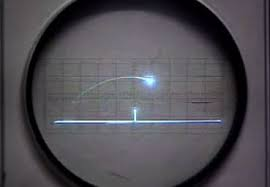
\includegraphics[width=0.5\linewidth]{img/Tennis_For_Two.jpg}
    \caption{Tennis For Two}
    \label{fig:Tennis}
\end{figure}

However, continuous advancements in hardware and software have significantly enhanced the quality and complexity of gaming experiences.
\\
The introduction of dedicated graphics processing units (GPUs) enabled the development of three-dimensional environments and more realistic rendering, increasing so the attractiveness of video games to a broader audience. Furthermore, as said before, the emergence of online gaming marked a fundamental shift in the industry, allowing users to interact in real time and creating network effects that contributed to the expansion of the user base \cite{esa2024, nvidia_raytracing,intel_gpu}.\\
More recent innovations, such as cloud gaming and artificial intelligence, have further reduced entry barriers and improved user engagement. Cloud gaming, in particular, allows users to access high-quality games without the need for advanced hardware, while AI technologies enhance gameplay through adaptive environments and personalized experiences \cite{redbull_ai_gaming, xbox_cloud_gaming}.\\
Overall, these technological advancements have not only improved product quality but have also contributed to the expansion of the market and the increase in industry revenues.


\subsubsection{Mobile Gaming}
Mobile gaming represents one of the most significant drivers of expansion in the video game industry over the past decade. The widespread diffusion of smartphones has substantially lowered entry barriers, allowing a much broader segment of the population to access video games.
\\
According to \cite{esa2024}, a large proportion of gamers engage with video games through mobile devices, with usage rates reaching approximately 78.8\% across different age groups in the United States. This highlights the role of mobile platforms in expanding the user base beyond traditional console and PC gamers.
\\
From an economic perspective, mobile gaming has contributed to industry growth by increasing market size and enabling new forms of monetization, particularly through free-to-play models and in-app purchases.
\\\\

\subsubsection{New Business Models}
Another key factor behind the growth of the video game industry is the evolution of business models, which has significantly transformed the way revenues are generated. Traditionally, video games were primarily distributed through a pay-to-play model, where users purchased a game once and retained full access. \\
However, the industry has progressively shifted towards more flexible and diversified monetization strategies. The emergence of freemium models, for example, allows users to access games for free while generating revenues through in-game purchases, such as cosmetic items or gameplay enhancements. This approach has proven particularly effective in expanding the user base while maintaining strong revenue streams (with most performative games generating a revenue per user comprehended in the interval between \$1-\$5 \cite{freemium_game_models}). \\
Additionally, downloadable content (DLC) and expansion models have enabled firms to extend the lifecycle of games, generating continuous revenues beyond the initial sale. Subscription-based services, such as platform-specific gaming passes, have further reinforced recurring revenue streams by offering access to large libraries of games for a fixed periodic fee \cite{xbox_game_pass} \cite{playstation_plus}. \\
Other monetization strategies include advertising-based models, particularly common in mobile gaming, and loot box systems, which introduce randomized rewards and have been widely discussed in the literature due to their similarities to gambling mechanisms \cite{LootBox_Model}.\\
\\\\

\subsubsection{Social Effect}
Social dynamics represent another driver of growth --that is worth to mention-- in the video game industry, particularly through the presence of network effects. The value of many video games, in fact, increases as the number of users expands, especially in multiplayer and online environments.
\\
In this context, digital platforms such as Twitch and YouTube have played a crucial role in amplifying the visibility of video games, allowing content creators to reach large audiences and influence consumer behavior. This form of indirect promotion has contributed to the rapid diffusion of games across different segments of the population.\\
In fact, according to statistics, more than 40\% of players discover new games through streams, giving even small studios a chance to rise in the charts without huge budgets if their game is noticed and shown by a popular content creator \cite{streaming_game_popularity} \cite{impact_game_streaming_industry}. \\
For many viewers it is more interesting to watch the stream than to run the game alone. Thus, the popularity of the game can be measured not only by the number of active players, but also by the number of hours of viewing \cite{streaming_game_popularity} .
\\
From an economic perspective, these mechanisms reinforce demand by creating positive feedback loops, where increased visibility leads to higher adoption rates, which in turn enhances the attractiveness of the product.

 

\subsubsection{The core reason because people play video games}

Understanding the underlying motivations that drive individuals to engage with video games is essential to explain the sustained growth in demand. Video games provide a combination of entertainment, cognitive stimulation, and social interaction, making them an attractive form of leisure activity across different demographic groups.
\\
Empirical evidence supports this view. According to \cite{esa2024} \ref{fig:Why_People_Play_Videogames}, a large portion of players report that gaming contributes positively to their cognitive and social skills. For instance, 73\% of gamers believe that video games improve problem-solving abilities, while 64\% associate gaming with enhanced teamwork and collaboration skills.\\
These factors contribute to the persistence of demand over time, reinforcing the position of video games as a central component of modern digital entertainment.

 
\begin{figure} [H]
    \centering
    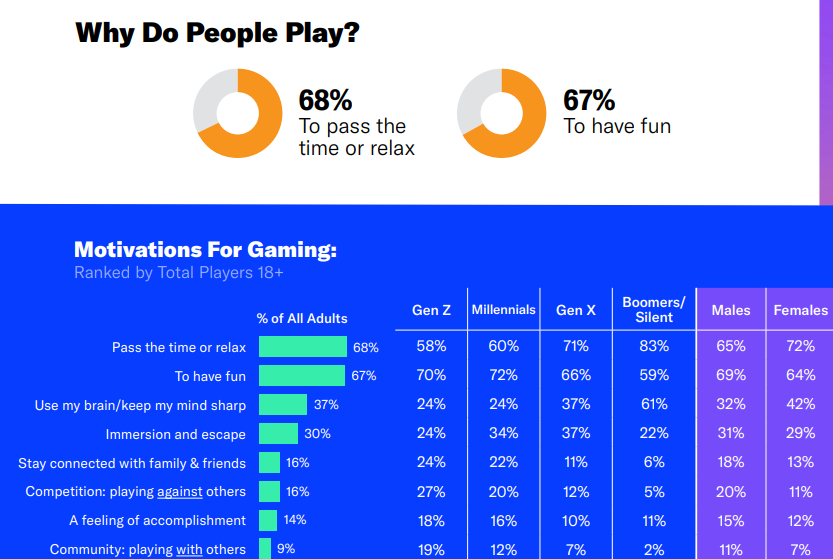
\includegraphics[width=0.5\linewidth]{img/Why_People_Play_Videogames.png}
    \caption{Why people play video games}
    \label{fig:Why_People_Play_Videogames}
\end{figure}




\subsection{The market}
The video game market has undergone significant structural changes over the past decades, characterized by a substantial expansion of its user base. The increasing diffusion of online gaming has played a central role in this transformation. According to \cite{esa2024}, the share of players engaging in online gaming in the United States increased from approximately 18\% in 1999 to nearly 90\% in recent years, highlighting the growing importance of connectivity in modern gaming experiences.\\
In addition, the demographic composition of the gaming population has become increasingly diversified. Contrary to the traditional perception of video games as a form of entertainment primarily targeted at younger audiences, recent data indicate that a large proportion of adults actively engage in gaming activities \ref{fig:Grafico_ESA}. This shift has contributed to a broader and more stable demand base.  
\begin{figure} [H]
    \centering
    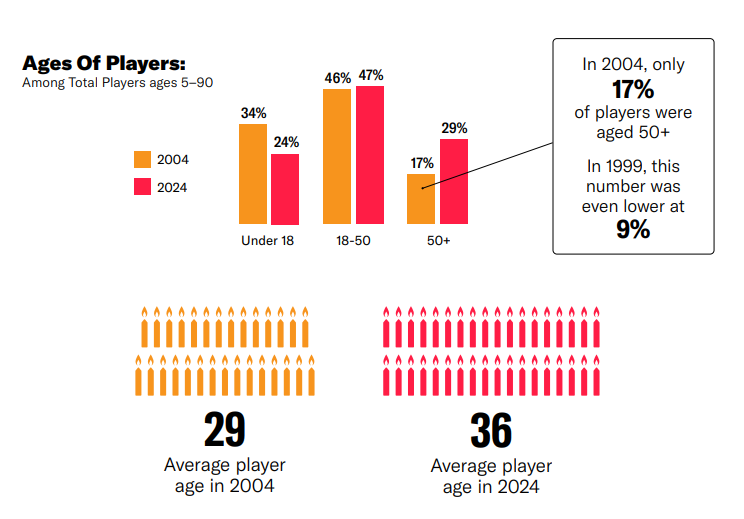
\includegraphics[width=0.5\linewidth]{img/Screenshot 2026-05-02 010839.png}
    \caption{Graph from ESA 2024}
    \label{fig:Grafico_ESA}
\end{figure}
Furthermore, gender distribution within the gaming population has become increasingly balanced, suggesting that video games have evolved into a mass-market form of entertainment rather than a niche activity. These structural changes in the user base have played a key role in supporting the long-term growth of industry revenues \ref{fig:Males and Females}. 

\begin{figure} [H]
    \centering
    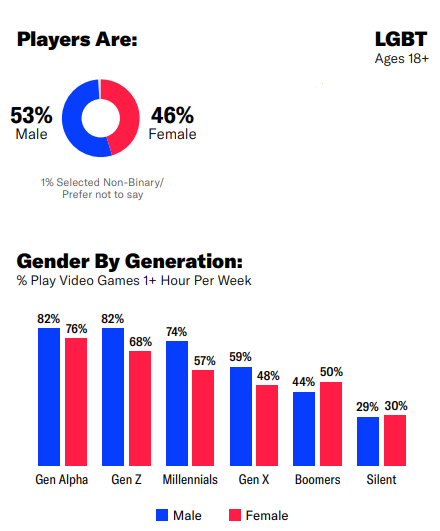
\includegraphics[width=0.5\linewidth]{img/Grafico_ESA_MF.png}
    \caption{Males and Females in Video games}
    \label{fig:Males and Females}
\end{figure}

\subsection{The purpose of this project}
While the video game industry has experienced strong structural growth over the past decades, understanding the drivers behind this expansion requires distinguishing between long-term economic and technological factors and short-term shocks such as the COVID-19 pandemic. The pandemic can be interpreted as a temporary demand shock that significantly accelerated industry revenues, followed by a period of normalization after 2021.

In this context, this study aims to analyze the evolution of video game industry revenues over the period 2014–2024, identifying the key macroeconomic and socio-demographic determinants of growth. In particular, the analysis focuses on variables such as income levels, inequality, population size, mental health indicators, and government restrictions during the pandemic period, in order to assess their impact on industry performance.

 

%*******************************************************
% Chapters
%*******************************************************
%\mainmatter

% Do not edit
%\renewcommand{\chaptermark}[1]{\markboth{\MakeUppercase{\chaptername\ \thechapter.\ #1}}{}}

% Add more \input{} commands as needed. Chapters can all be
% contained in one single .tex file, or you can have one file
% per chapter.

\chapter{Literature Review}

Several articles have conducted research closely related to ours, 
and will be referenced throughout this chapter: both for their 
theoretical contributions and, in some cases, for data or figures 
that would otherwise have been inaccessible to us.\\

\cite{chang2021videogame_pandemic} examined the impact of COVID-19 
on the amount of time users spent playing video games, drawing data 
from \cite{steamdb} — an independent database covering the entire 
Steam catalog, providing player charts, price history, update 
histories, and detailed product data. Steam itself is the world's 
largest digital distribution platform for PC games, developed by 
Valve Corporation, allowing users to purchase, download, and manage 
games from a centralized library \cite{steam_about}.\\

This article provides a particularly relevant figure, showing 
differences in playtime — across the 500 most popular games at the 
time — between 2019 and 2020.\\

\begin{figure}[H]
    \centering
    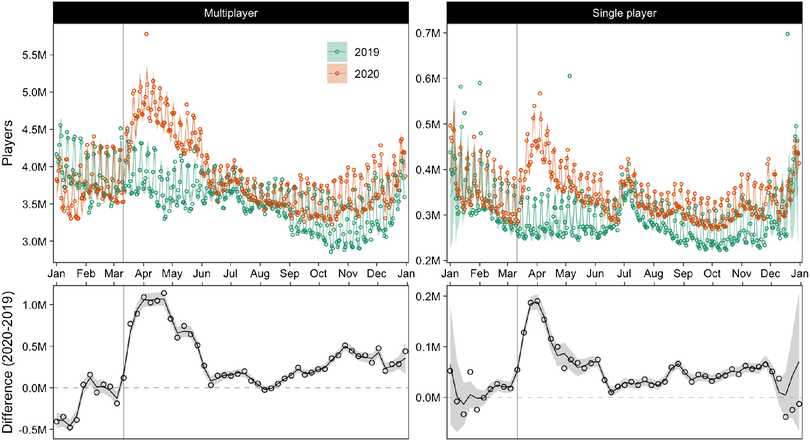
\includegraphics[width=\textwidth]{img/COVID_Steam_Players_Increase.png}
    \caption{Steam players comparison 2019--2020\\
    Note: the vertical gray line marks March 11th, 2020, 
    when the WHO officially declared COVID-19 a pandemic.\\
    Source: \cite{chang2021videogame_pandemic, steamdb}}
    \label{fig:Steam_Players_Increase_COVID1}
\end{figure}
A clear COVID-related effect is visible in the time series, with a 
marked peak between March and May 2020. Notably, the spike in 
multiplayer games persisted longer than that of single-player titles, a pattern that likely reflects users' need to maintain social 
interaction and compensate for the loss of in-person contact during 
lockdown periods.\\
This interpretation finds support in \cite{gaming_disorder_covid}, 
which examined both the adaptive and maladaptive dimensions of video 
game use as a coping strategy during the pandemic. While moderate 
gaming may represent a healthy way to spend time and socialize, excessive use carries the risk of developing into the so-called "gaming disorder". The World Health Organization defines gaming disorder as a pattern of behavior 
characterized by impaired control over gaming, the progressive 
prioritization of gaming over other activities, and its continuation 
despite negative consequences \cite{who_gaming_disorder}. 
\cite{gaming_disorder_covid} further argue that this risk was 
heightened during the pandemic, as many alternative coping 
strategies became unavailable, while opportunities to play -- at any 
hour — increased significantly.\\
The relationship between intensive gaming and mental health is 
explored further in \cite{heavy_gaming&depression}, which finds that 
adolescents classified as heavy gamers reported more depressive 
symptoms than their coetaneous. \cite{gentile2011pathological_gaming} 
refines this picture by highlighting the role of timing, stating that among 
emerging adults aged between 18 and 22 years, habitual late-night gaming (after 2 AM) was associated with heightened vulnerability. This is consistent with \cite{gaming_disorder_covid}'s observation that, as teenagers were free from school schedules (at least at the beginning), they were more likely to extend their gaming sessions into the night.\\
Taken together, this body of literature supports the inclusion of 
depression rates and COVID-related elements (such as Stringency Index) among the variables considered in our analysis, given its documented association with patterns of excessive gaming.


\chapter{Model}
\paragraph{What Model Was Used}
The model used for this research was a Generalized Additive Model (GAM) with random intercepts.
To explain what a GAM with random intercepts is, we first have to introduce some lower-level models.\\
\section{From LM to GLM to GAM to GAM + re}
Linear regression is a method used to describe how the average 
value of a numerical outcome changes according to a linear 
combination of predictors.
This kind of regression can be used to represent relationships 
between variables.
However, the linear regression model relies on several strong assumptions, 
in particular that the response variable is continuous, 
normally distributed, and linearly related to the predictors. 
In many real-world applications, these assumptions are not appropriate. 
As in our case our outcome is non-normally distributed, we need
to use a different model.
\subsubsection{Linear Model (LM)}
\begin{equation}
Y_i = \beta_0 + \beta_1x_{i1} + \cdots + \beta_px_{ip} + \varepsilon_i,
\end{equation}

where

\begin{equation}
\varepsilon_i \sim N(0,\sigma^2).
\end{equation}

and:
\begin{itemize}
    \item $Y_i$ is the response variable;
    \item $\beta_0$ is the intercept;
    \item $\beta_1,\ldots,\beta_p$ are the regression coefficients associated with the predictors;
    \item $x_{i1},\ldots,x_{ip}$ are the values of the predictors for observation $i$;
    \item $\varepsilon_i$ is the random error term, assumed to be independently and identically distributed as
    \[
    \varepsilon_i \sim N(0,\sigma^2).
    \]
\end{itemize}\\
\small Source: \textcite[p.~37]{gelman2007book}

\subsection{From LM to GLM}
To address these above-mentioned limitations, we can resort to 
the Generalized Linear Model (GLM), which extends the classical
linear model by allowing the response variable to follow 
distributions from the exponential family and by introducing a 
link function that connects the expected value of the response 
to the linear predictor.
\subsubsection{Generalized Linear Model (GLM)}

\begin{equation}
g(\mu_i)=
\beta_0+\beta_1x_{i1}+\cdots+\beta_px_{ip},
\end{equation}

where

\begin{equation}
\mu_i=E(Y_i),
\end{equation}

and:
\begin{itemize}
    \item $\mu_i=E(Y_i)$ is the expected value of the response variable;
    \item $g(\cdot)$ is the link function;
    \item $\eta_i$ denotes the linear predictor.
\end{itemize}\\
\small Source: \textcite[p.~109]{gelman2007book}

\subsection{From GLM to GAM}
While GLMs provide a flexible framework for handling different
types of response variables, they still assume a linear 
relationship between the transformed expected value of the
response and the predictors. In practice, this assumption would
still be too restrictive, since many relationships in real 
data are non-linear.\\
To overcome this limitation, Generalized Additive Models (GAMs) 
extend GLMs by allowing the linear predictor to include smooth, 
functions of the covariates. This makes it possible to model 
complex and potentially non-linear effects of predictors on the 
response variable while maintaining interpretability.
\subsubsection{Generalized Additive Model (GAM)}

\begin{equation}
g(\mu_i)=
\beta_0+
f_1(x_{i1})+
f_2(x_{i2})+
\cdots+
f_p(x_{ip}) +
\varepsilon_i,
\end{equation}

where $f_j(\cdot)$ are smooth functions estimated from the data.\\
\small Source: \textcite[p.~307]{james2021islr}

\subsection{From GAM to GAM + re}
Although GAMs allow for flexible functional forms, standard models assume that 
all observations are independent. In our case, however, the data points are 
grouped by continent. Observations belonging to the same continent might share unobserved characteristics 
not captured by the other predictors, which could violate this assumption of 
independence.\\
To account for this shared structure, we included a random intercept for the 
continent variable directly within the GAM framework. In R, this is implemented 
using a random effect smooth basis (\texttt{bs = "re"}). This approach allows 
the model to estimate and control for baseline differences across continents, 
adjusting for the fact that data within the same continent may be correlated, 
while still accurately capturing the non-linear relationships of the other 
variables.

\subsubsection{Generalized Additive Model with Random Intercepts (GAM + re)}
\begin{equation}
g(\mu_i) = \beta_0 + \sum_{j=1}^{p}f_j(x_{ij}) + \mathbf{Z}_i\mathbf{b} + \varepsilon_i
\end{equation}
where:
\begin{itemize}
    \item $\mathbf{Z}_i$ is the design matrix row associated with the random effects;
    \item $\mathbf{b}$ is the vector of random effects, assumed to be normally distributed as $\mathbf{b} \sim N(\mathbf{0}, \mathbf{D})$.
\end{itemize}
In our specific formulation, $\mathbf{b}$ reduces to a single random intercept per 
continent, and the covariance matrix $\mathbf{D}$ simplifies to a single scalar 
variance component $\sigma^2_{\text{continent}}$, since no random slopes or nested 
grouping structures are included in the model.\\
\small Source: \textcite[p.~307]{james2021islr} for GAM model and \textcite[p.~105]{zuur2009mixed_effects_models} for the random-effects component $\mathbf{Z}_i\mathbf{b}$.


\subsection{Model Specification for This Study}
Initial models using a Gaussian family on the original scale 
yielded poor goodness-of-fit, with negative adjusted $R^2$ values. 
Given the positive and right-skewed distribution of video game 
sales, a Gamma family with log link was initially considered as 
a more appropriate distributional assumption \cite{hosch2026gamma}. 
However, applying a log transformation to the response variable 
substantially improved residual behaviour and approximated 
normality, making a Gaussian family with log transformed sales, 
the most appropriate specification for the final model:

\begin{equation}
Y_i^* = \log(Y_i) \sim N(\mu_i, \sigma^2)
\end{equation}

where $Y_i$ represents video game sales in millions and $Y_i^*$ 
is the log-transformed response used in the final model.

\subparagraph{Formula of the Chosen Model}
\begin{equation}
\begin{aligned}
Y_i^* = \beta_0 + f_1(IU_i) + f_2(Year_i, DR_i) + f_3(U_i) + \beta_1 \cdot GNI_i + b_{c(i)} + \varepsilon_i
\end{aligned}
\end{equation}

where:

\begin{itemize}
    \item $Y_i$ denotes sales (in millions) for observation $i$;

    \item $\beta_0$ is the intercept term;
    
    \item $f_1(IU_i)$ represents the smooth nonlinear effect of Internet Users;
    
    \item $f_2(Year_i,DR_i)$ represents a joint nonlinear effect of Year and Depression Rates, modelled using a tensor product smooth;
    
    \item $f_3(U_i)$ represents the smooth nonlinear effect of Unemployment;
    
    \item $\beta_1$ represents the linear effect of GNI per capita;
    
    \item $b_{c(i)}$ is a continent-specific random effect;
    
    \item $\varepsilon_i$ is the error term, assumed to follow a normal distribution with mean zero and variance $\sigma^2$, i.e.,
    $\varepsilon_i \sim N(0,\sigma^2)$.
\end{itemize}

Below (Figure \ref{fig:Log_Model}) are the graphs of residuals of the chosen model, so after the log transformation.\\
Residual plots for the model prior to the log transformation are provided in the Appendix B (Figure \ref{fig:Non_Log_Model}).

\begin{figure}[H]
    \centering
    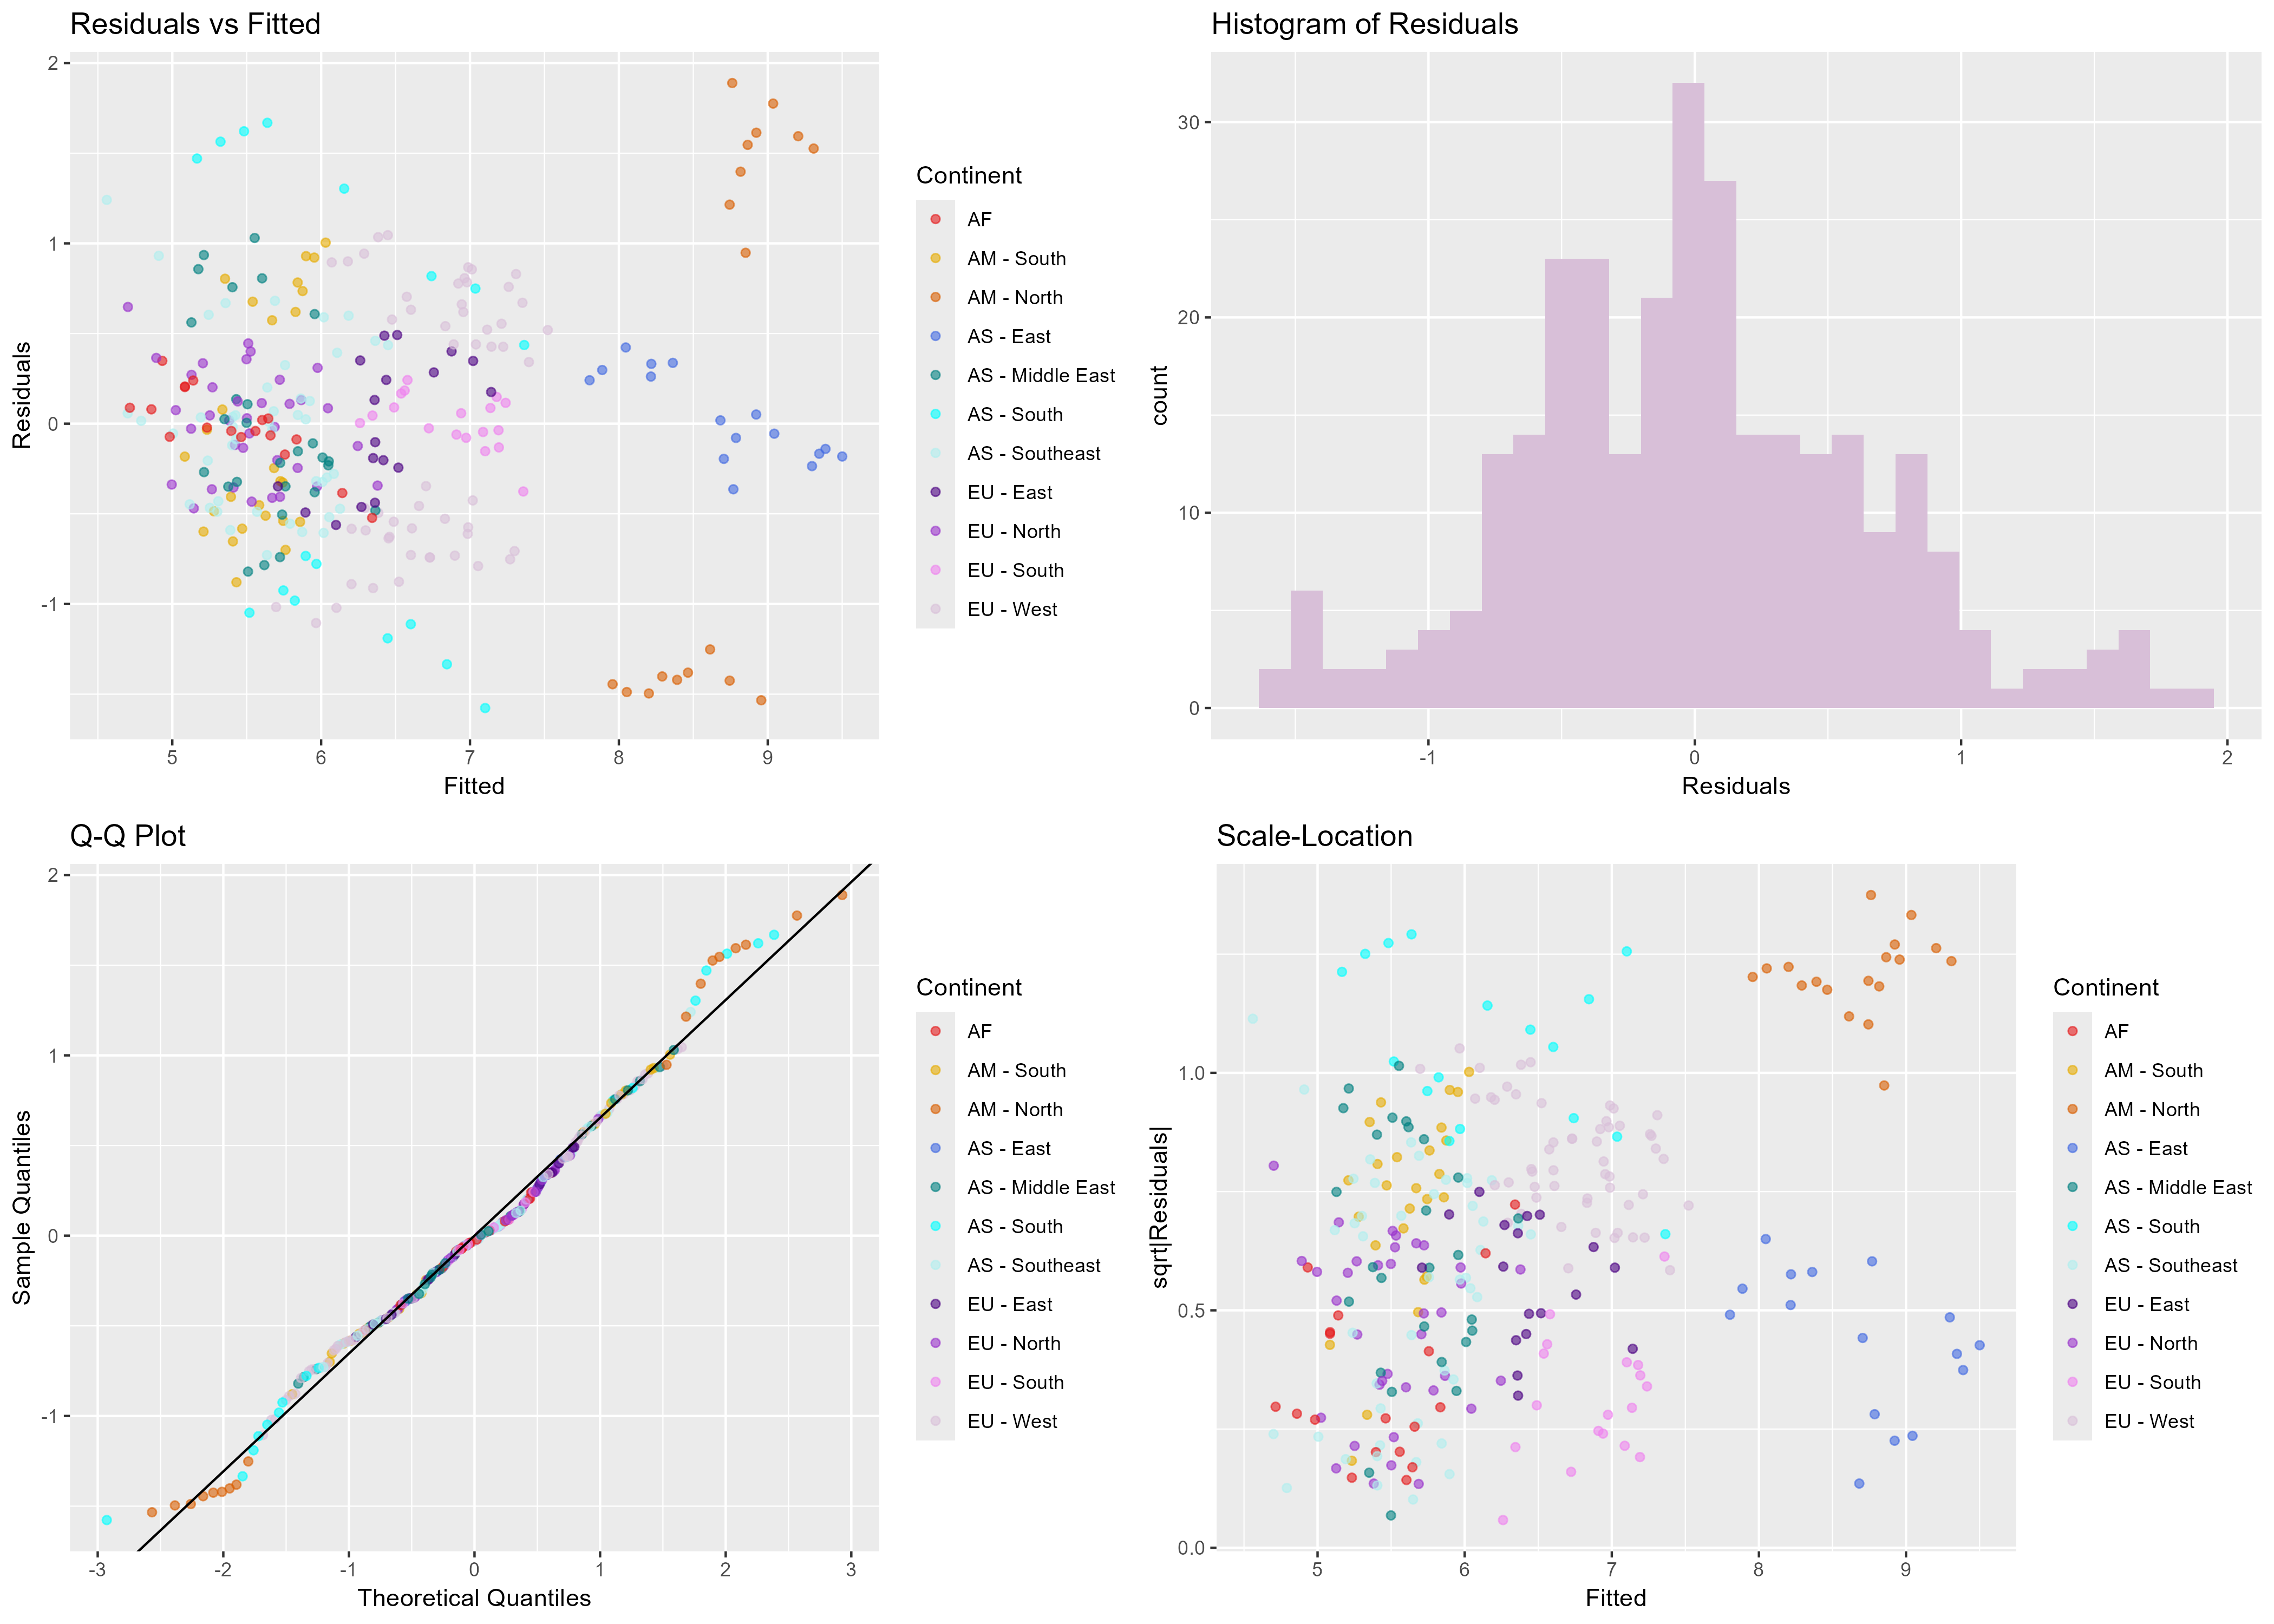
\includegraphics[width=\textwidth]{img/Log_Model_Colored_Graph.png}
    \caption{Diagnostic Residual Plots for the Log Model}
    \label{fig:Log_Model}
\end{figure}

\section{Model Results}
\begin{table}[H]
\centering
\caption{GAM + re Estimation Results}
\begin{tabular}{|l|c|c|c|c|}
\hline
\textbf{Variable} & \textbf{Estimate / edf} & \textbf{Std. Error / Ref.df} & \textbf{Statistic} & \textbf{p-value} \\
\hline\hline
\multicolumn{5}{|l|}{\textit{Parametric terms}} \\
\hline
Intercept & 6.860 & 0.417 & 16.469 & $<0.001^{***}$ \\
$GNI_i$ & $-1.072 \times 10^{-5}$ & $4.287 \times 10^{-6}$ & $-2.502$ & $0.013^{*}$ \\
\hline\hline
\multicolumn{5}{|l|}{\textit{Smooth terms}} \\
\hline
$f_1(IU_i)$ & 3.232 & 4.072 & 4.463 & $0.002^{**}$ \\
$f_2(Year_i,DR_i)$ & 6.522 & 6.898 & 10.261 & $<0.001^{***}$ \\
$f_3(U_i)$ & 2.346 & 2.977 & 4.736 & $0.003^{**}$ \\
$b_{c(i)}$ & 9.730 & 10.000 & 50.250 & $<0.001^{***}$ \\
\hline\hline
\multicolumn{5}{|l|}{\textit{Model fit}} \\
\hline
Adjusted $R^2$ & \multicolumn{4}{l|}{0.717} \\
Deviance explained & \multicolumn{4}{l|}{73.9\%} \\
REML & \multicolumn{4}{l|}{349.39} \\
$n$ & \multicolumn{4}{l|}{293} \\
\hline
\end{tabular}
\\[0.5em]
\small Significance codes: $^{***}p<0.001$, $^{**}p<0.01$, $^{*}p<0.05$
The complete R model specification is provided in Appendix C (Model \ref{lst:gam}).\\
Note: as it is possible to see, all the model's variables are
statistically significant. This is due to the fact that
non significant variables (e.g. Stringency Index), have been
removed in order to guarantee a parsimonious and efficient model.
\end{table}

The intercept is equal to 6.860, number that represents the 
baseline log sales value when all the other variables are equal
to 0.\\
GNI per Capita shows a linear and statistically significant negative effect 
on sales with an estimate of $-1.072 \times 10^{-5}$, 
suggesting that, all else being equal, higher national income 
is associated with slightly lower video game sales.
\begin{figure}[H]
    \centering
    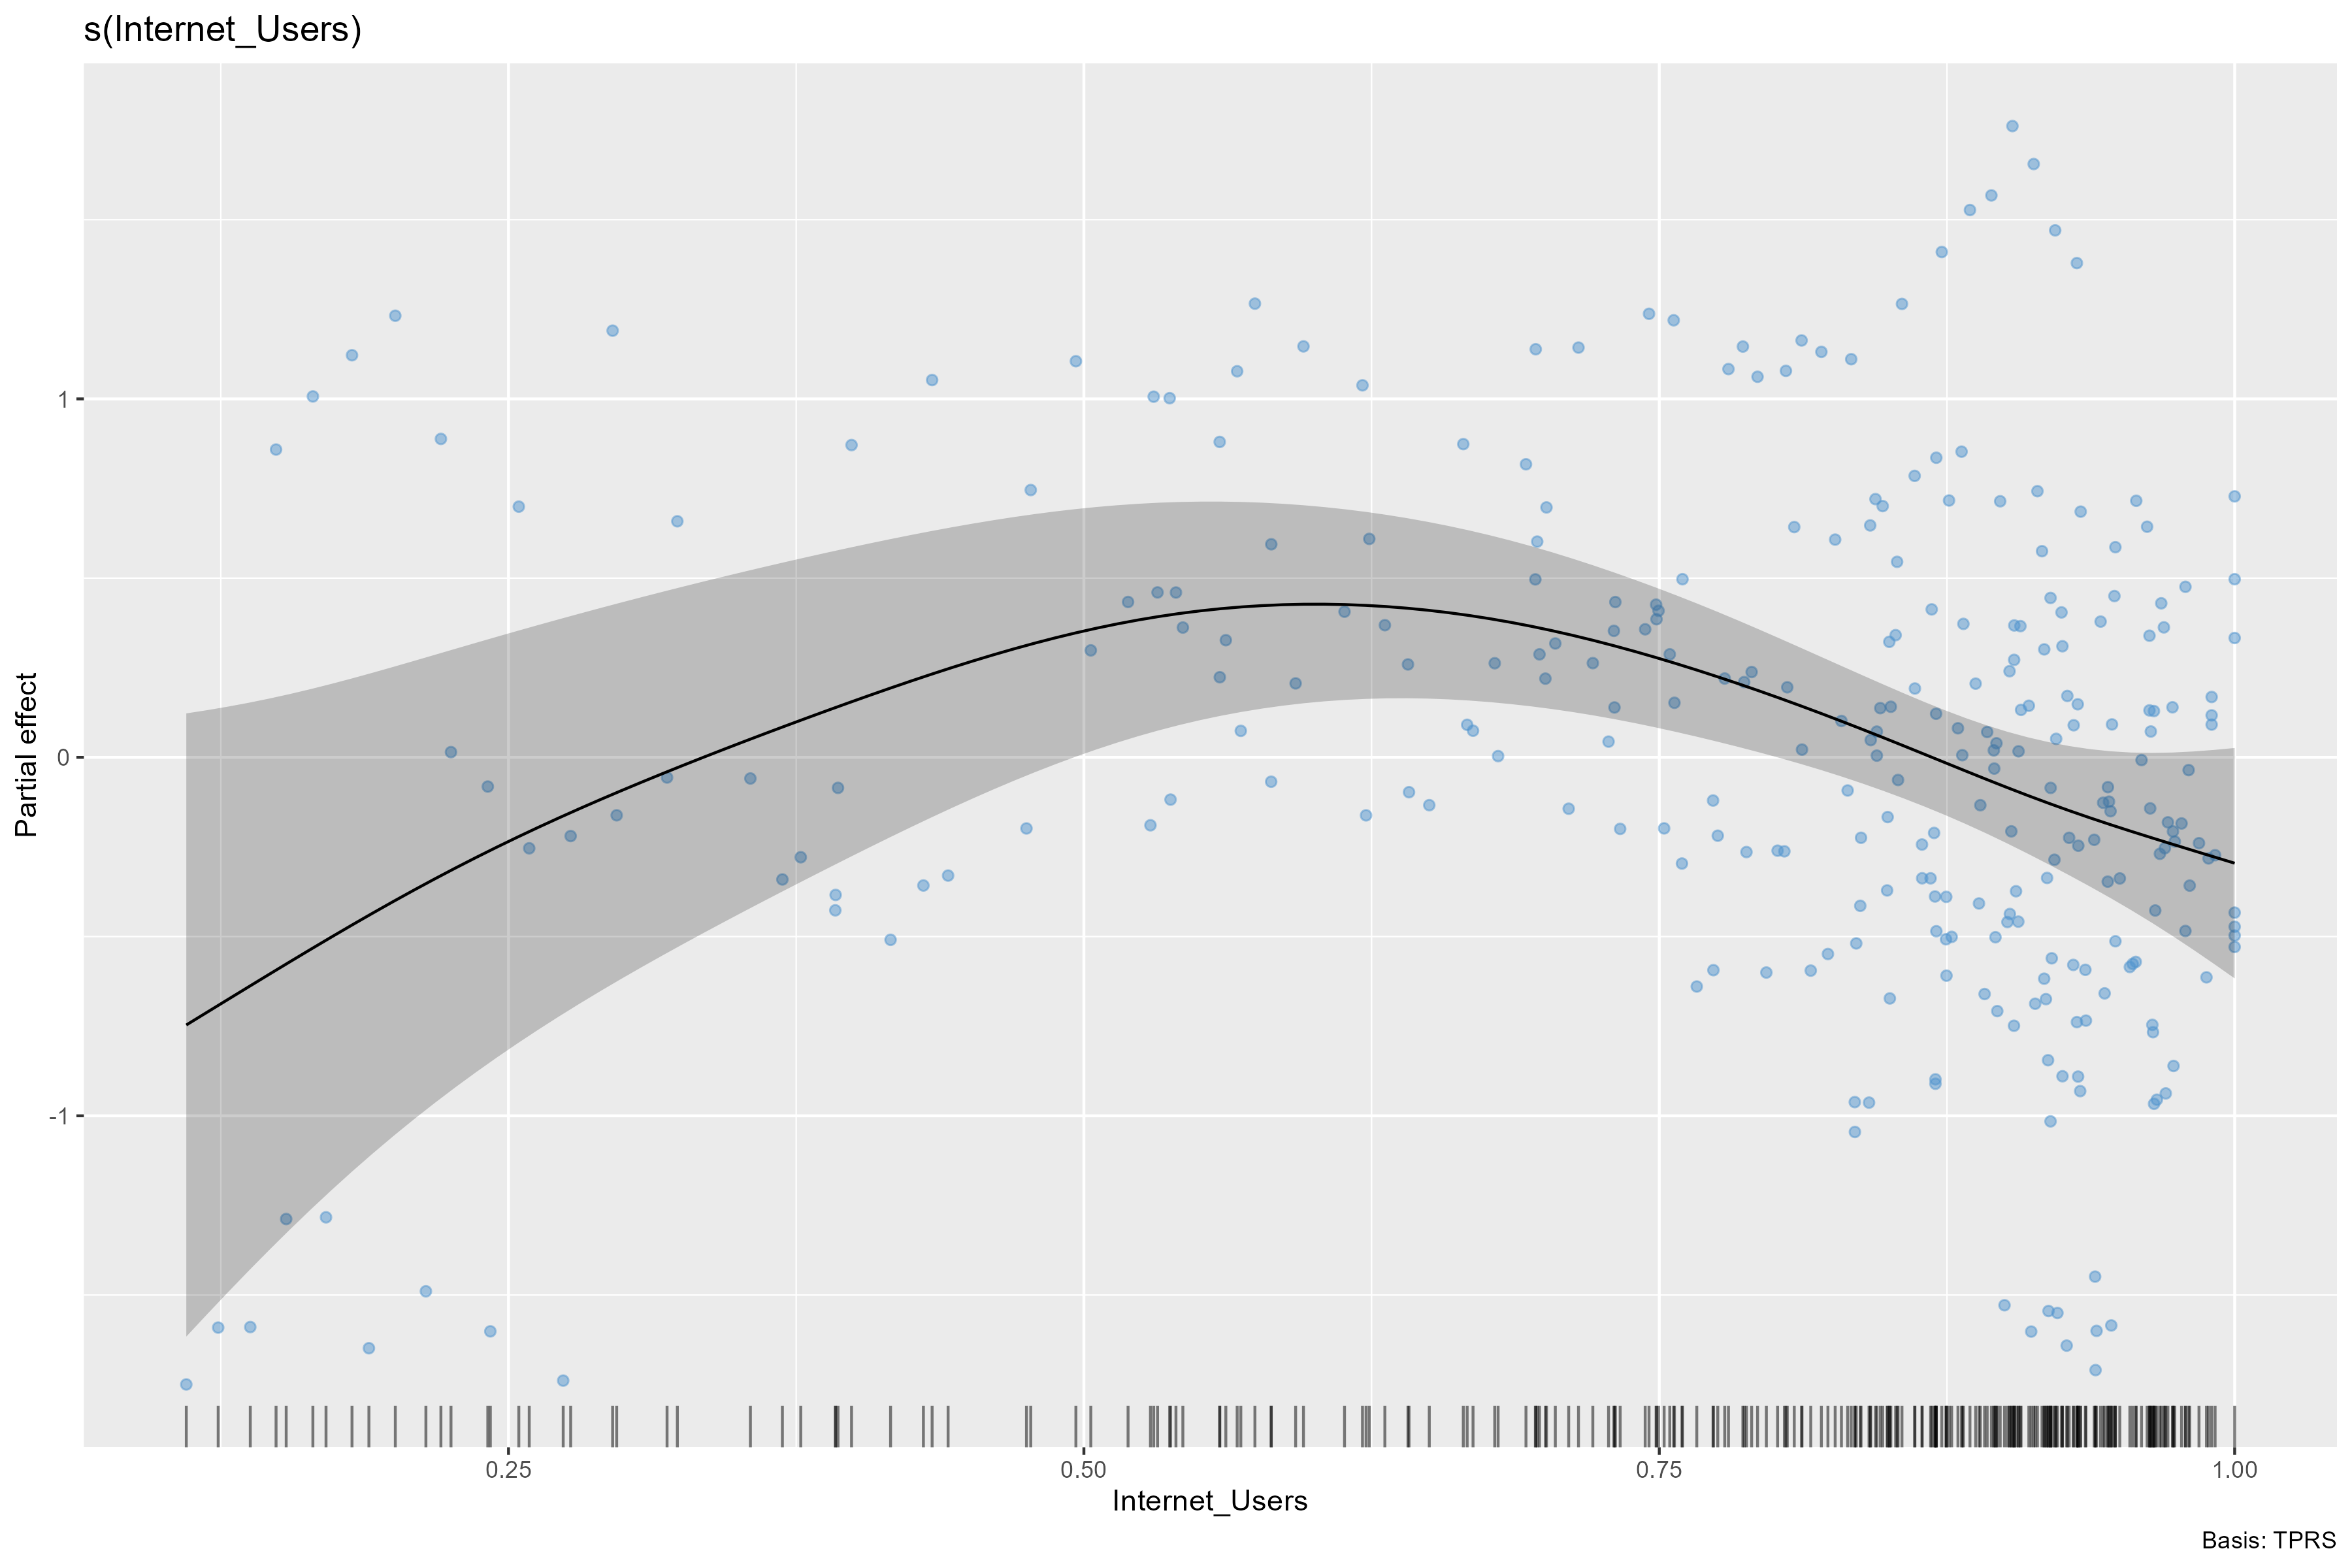
\includegraphics[width=\textwidth]{img/s_Internet_Users.png}
    \caption{Estimated partial effect of Internet Users on log(Sales)}
    \label{fig:s_Internet_Users}
\end{figure}
Internet Users exhibit a non-linear 
effect with an effective degrees of freedom (edf) value of 3.232 
suggesting a moderately flexible relationship (values of edf 
greater than 1 indicate nonlinear effects, with higher values 
reflecting greater functional flexibility).\\
While here the observations are more spread, the confidence 
interval is narrowest in the 0.75–1 range, where the rug plot 
confirms the highest concentration of observations, while it 
remains wide for the first three quarters of the spline where 
data are sparser.\\
A broader view shows that countries with 
intermediate internet penetration tend to be associated with 
higher sales in the video game market, while both less and more 
digitalized countries show a lower partial effect.\\
One possible explanation for the decline at high penetration rates is that 
in highly digitalized countries internet access extends across 
all age groups, including older demographics that may on average 
be less inclined to spend money on video games, though caution 
is needed in drawing causal conclusions from an observational 
model.
\begin{figure}[H]
    \centering
    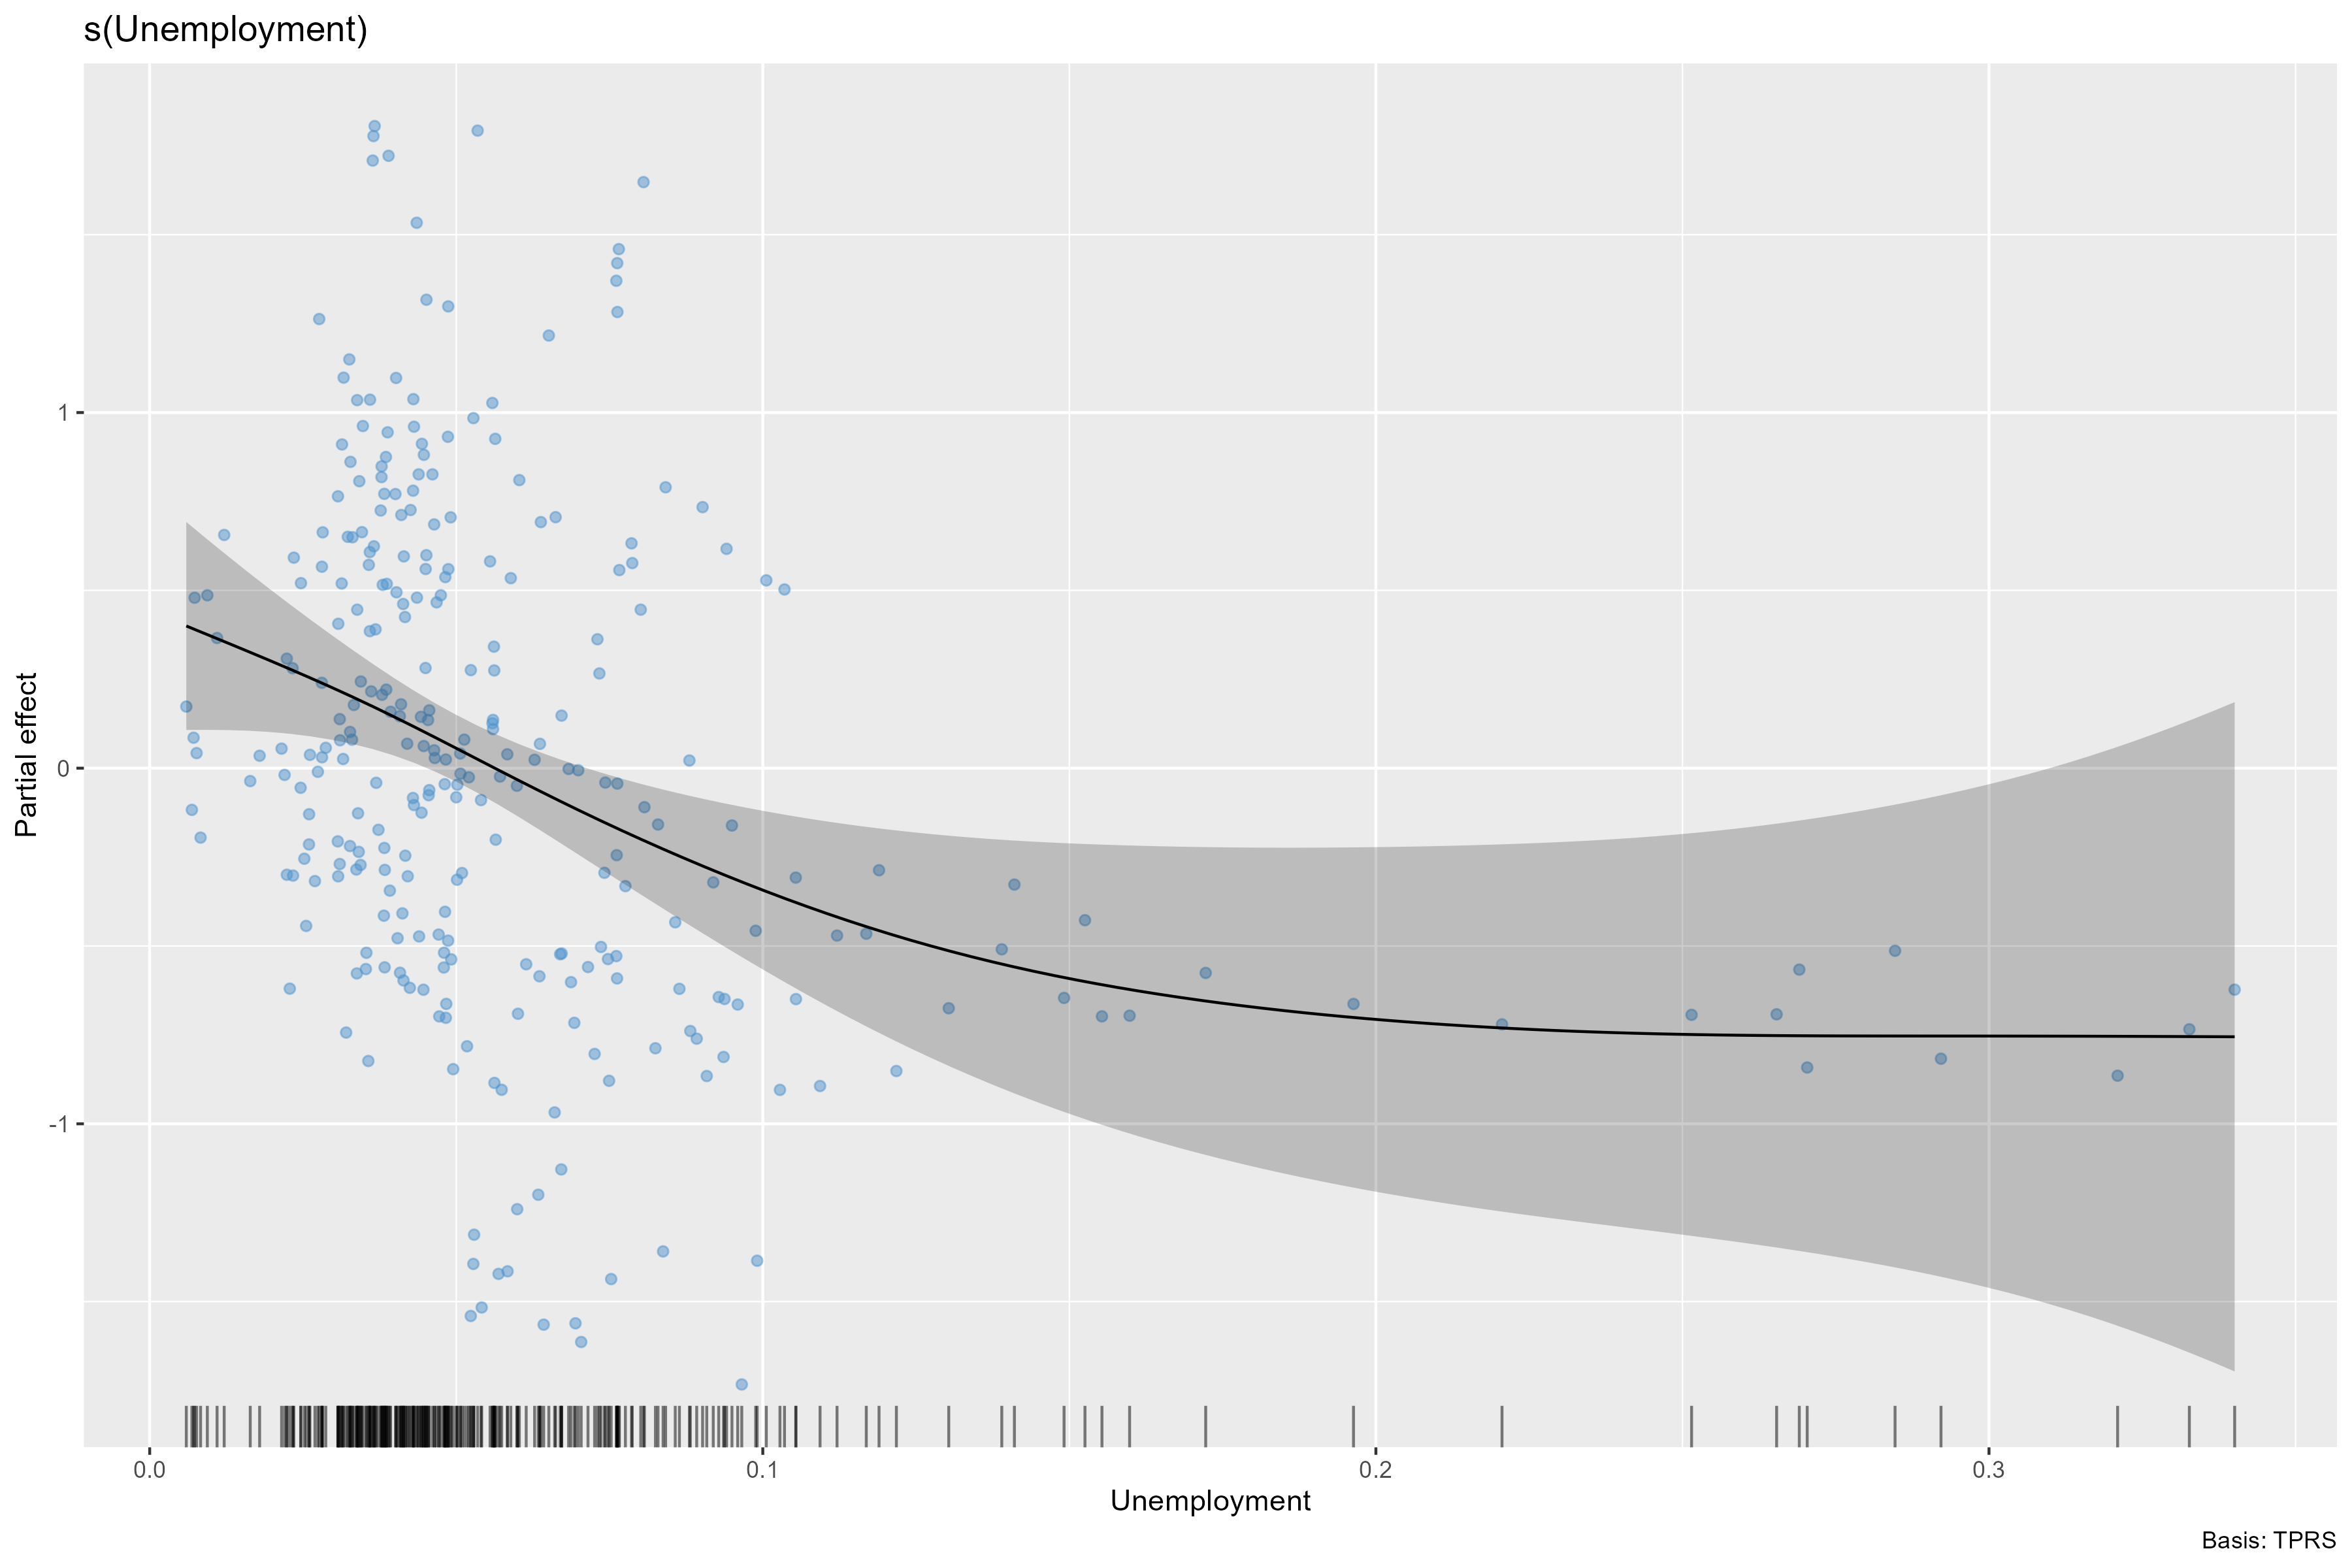
\includegraphics[width=\textwidth]{img/s_Unemployment.png}
    \caption{Estimated partial effect of Unemployment Rates on log(Sales)}
    \label{fig:s_Unemployment}
\end{figure}
Similarly, Unemployment displays a similar pattern, with an edf of 2.346
indicating a moderately flexible non-linear trend.\\
Unemployment's effect on our response variable (log(Sales)) 
starts from positive values when unemployment is near 0 and goes 
decreasing as unemployment increases.\\
It is important to notice 
that, as the vast majority of the observations are concentrated 
in a small range (0–0.1), this interval is the one with more 
statistical evidence of the effect (having a narrower confidence 
interval), while there are too few observations of unemployment 
values higher than 0.1, leading us to be more skeptical about 
the spline in that part.\\
Note that these represent partial 
effects, meaning all other variables in the model are held 
constant.
\begin{figure}[H]
    \centering
    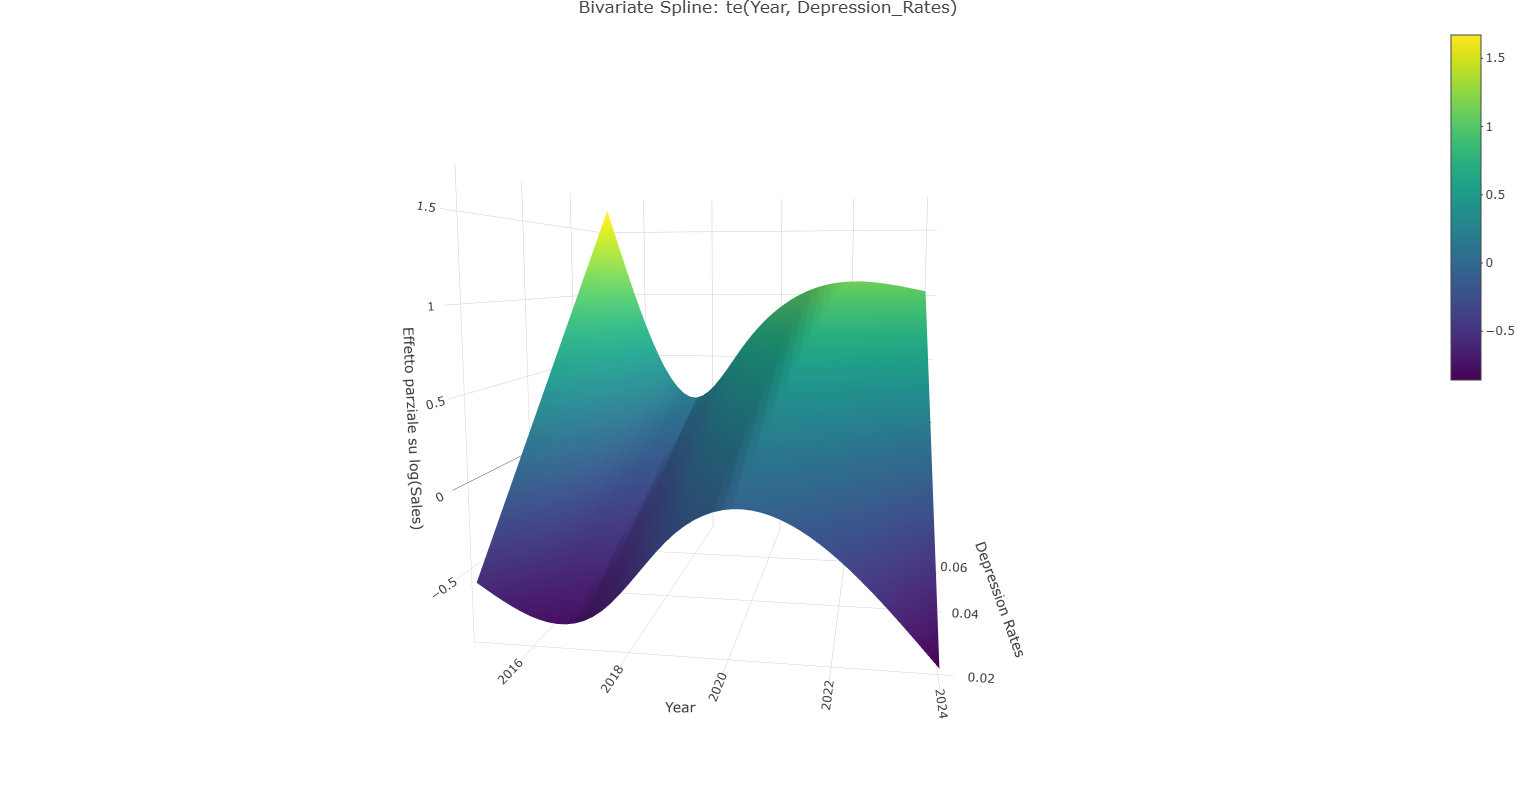
\includegraphics[width=\textwidth]{img/3D_Plot.png}
    \caption{3D visualization of the partial effect of $f_2(Year_i,DR_i)$ on log(Sales)}
    \label{fig:3D_Plot}
\end{figure}
The tensor product between Year and Depression Rates shows --
with an edf of 6.522 -- a strongly non linear and complex effect
of depression rates over sales, that is not constant over the years.\\
Overall, across all years, low depression rates are associated with lower sales, while higher 
depression rates tend to be associated with higher sales; even if it is important to remember that this refers to the 
partial effect, meaning all other variables in the model are held constant.\\
However, in the 2019–2022 period we can notice how depression rates start to have a stronger 
influence on the response variable, which could reflect a real-world effect tied to COVID-19:
rising depression rates coinciding with a boom in video games sales.
As for the spike around 2015-2016 at high depression rates, this is likely due to the scarcity 
of observations in that region of the data: where data points are few, the spline tends to 
behave in an unstable manner, producing estimates that are less reliable. This period should therefore be interpreted with caution.
\begin{figure}[H]
    \centering
    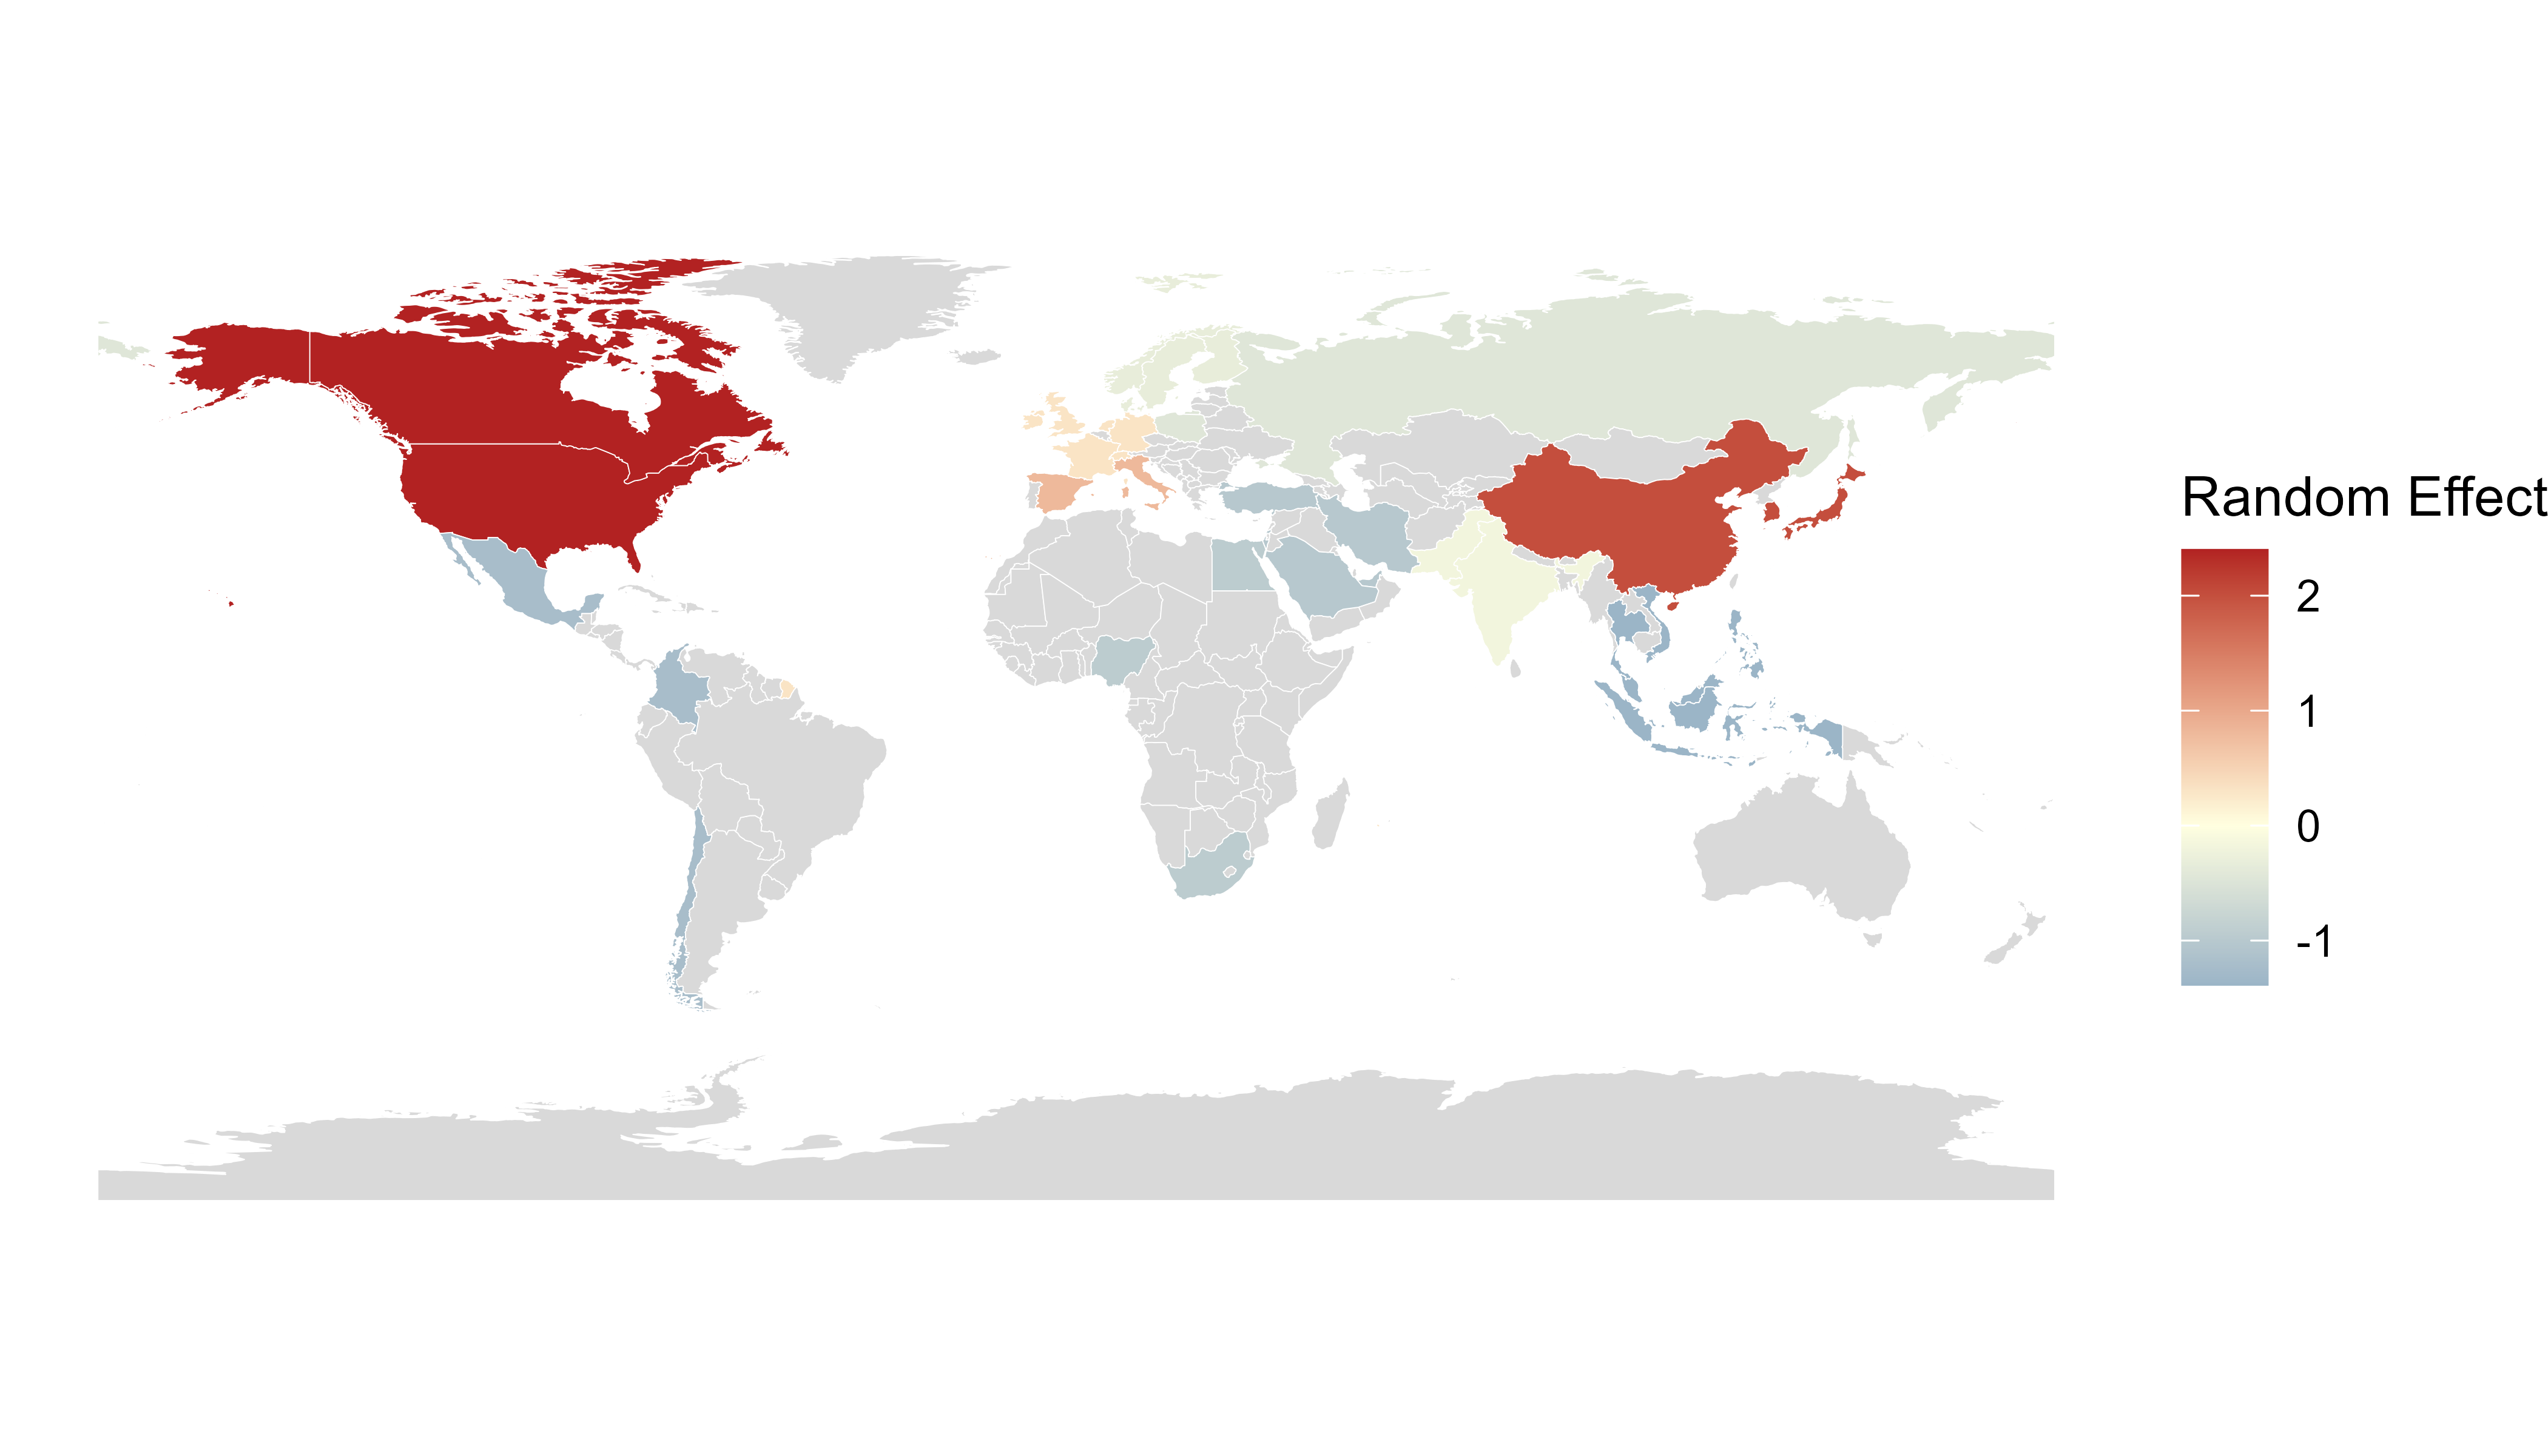
\includegraphics[width=\textwidth]{img/Random_Effect_Map.png}
    \caption{Random Effect Global Map}
    \label{fig:Random_Effect_Map}
\end{figure}
To conclude, to better illustrate the regional heterogeneity captured 
by the Continent term, the map visualizes the random effects estimated by the s(Continent, bs="re") term, capturing the residual variability in video game sales attributable to geographic location after accounting for all other covariates in the model. Countries shown in red exhibit systematically higher sales than what the other variables alone would predict, while countries in blue show the opposite pattern, and grey countries are absent from the dataset.
The most positive random effects are concentrated in North America and East Asia, which represent the world's historically dominant video game markets. Western Europe displays moderate positive effects, while Russia and Northern Europe show slight negative deviations.
The high edf of 9.730 for this term, approaching the maximum of 10, confirms the substantial regional heterogeneity captured by the model, with geography playing a meaningful role beyond what the continuous predictors can explain.
In general, the results indicate a strong overall fit, with an adjusted 
R-squared of 0.717 and a deviance explained of 73.9\%, 
suggesting that the model captures a substantial portion of the 
variability in sales.

%*******************************************************
% Conclusion
%*******************************************************
\chapter*{Conclusion}
% Do not edit
\addcontentsline{toc}{chapter}{Conclusion}
\label{chap:concl}
\markboth{CONCLUSION}{CONCLUSION}

\lipsum[1]

\section{Conclusion}

% ── Bibliography ────────────────────────────────────────────────
\clearpage
\phantomsection
\addcontentsline{toc}{chapter}{Bibliography}
%\bibliography{bib/Bibliography}
\printbibliography

% ── Appendices ──────────────────────────────────────────────────
\appendix
\chapter{Countries' Table}
This appendix presents the complete list of the 39 countries analyzed in the research, categorized by macro-region and sub-region.

\begin{longtable}{llp{6cm}}
\caption{List of the 39 selected countries by region.} \label{tab:selected_countries} \\
\toprule
\textbf{Country} & \textbf{ISO Code} & \textbf{Region / Sub-region} \\
\midrule
\endfirsthead

\caption[]{List of the 39 selected countries by region. (Continued)} \\
\toprule
\textbf{Country} & \textbf{ISO Code} & \textbf{Region / Sub-region} \\
\midrule
\endhead

\bottomrule
\endfoot

% ── AMERICAS ──────────────────────────────────────────────────
\multicolumn{3}{l}{\textbf{Americas}} \\
\midrule
Canada & CAN & Americas - North America \\
United States & USA & Americas - North America \\
Mexico & MEX & Americas - Latin America \\
Chile & CHL & Americas - Latin America \\
Colombia & COL & Americas - Latin America \\
\midrule

% ── AFRICA ────────────────────────────────────────────────────
\multicolumn{3}{l}{\textbf{Africa}} \\
\midrule
Egypt & EGY & Africa \\
Nigeria & NGA & Africa \\
South Africa & ZAF & Africa \\
\midrule

% ── ASIA ──────────────────────────────────────────────────────
\multicolumn{3}{l}{\textbf{Asia}} \\
\midrule
China & CHN & Asia - East Asia \\
Hong Kong & HKG & Asia - East Asia \\
Japan & JPN & Asia - East Asia \\
Republic of Korea & KOR & Asia - East Asia \\
India & IND & Asia - South Asia \\
Pakistan & PAK & Asia - South Asia \\
Indonesia & IDN & Asia - Southeast Asia \\
Malaysia & MYS & Asia - Southeast Asia \\
Philippines & PHL & Asia - Southeast Asia \\
Singapore & SGP & Asia - Southeast Asia \\
Thailand & THA & Asia - Southeast Asia \\
Vietnam & VNM & Asia - Southeast Asia \\
Iran & IRN & Asia - Middle East \\
Israel & ISR & Asia - Middle East \\
Saudi Arabia & SAU & Asia - Middle East \\
United Arab Emirates & ARE & Asia - Middle East \\
Turkey & TUR & Asia - Middle East \\
\midrule

% ── EUROPE ────────────────────────────────────────────────────
\multicolumn{3}{l}{\textbf{Europe}} \\
\midrule
Denmark & DNK & Europe - Northern Europe \\
Finland & FIN & Europe - Northern Europe \\
Norway & NOR & Europe - Northern Europe \\
Sweden & SWE & Europe - Northern Europe \\
France & FRA & Europe - Western Europe \\
Germany & DEU & Europe - Western Europe \\
Ireland & IRL & Europe - Western Europe \\
Netherlands & NLD & Europe - Western Europe \\
Switzerland & CHE & Europe - Western Europe \\
United Kingdom & GBR & Europe - Western Europe \\
Italy & ITA & Europe - Southern Europe \\
Spain & ESP & Europe - Southern Europe \\
Poland & POL & Europe - Eastern Europe \\
Russian Federation & RUS & Europe - Eastern Europe \\

\end{longtable}
\setstretch{1.5}
\chapter{Supplementary Material}
\begin{figure}[H]
    \centering
    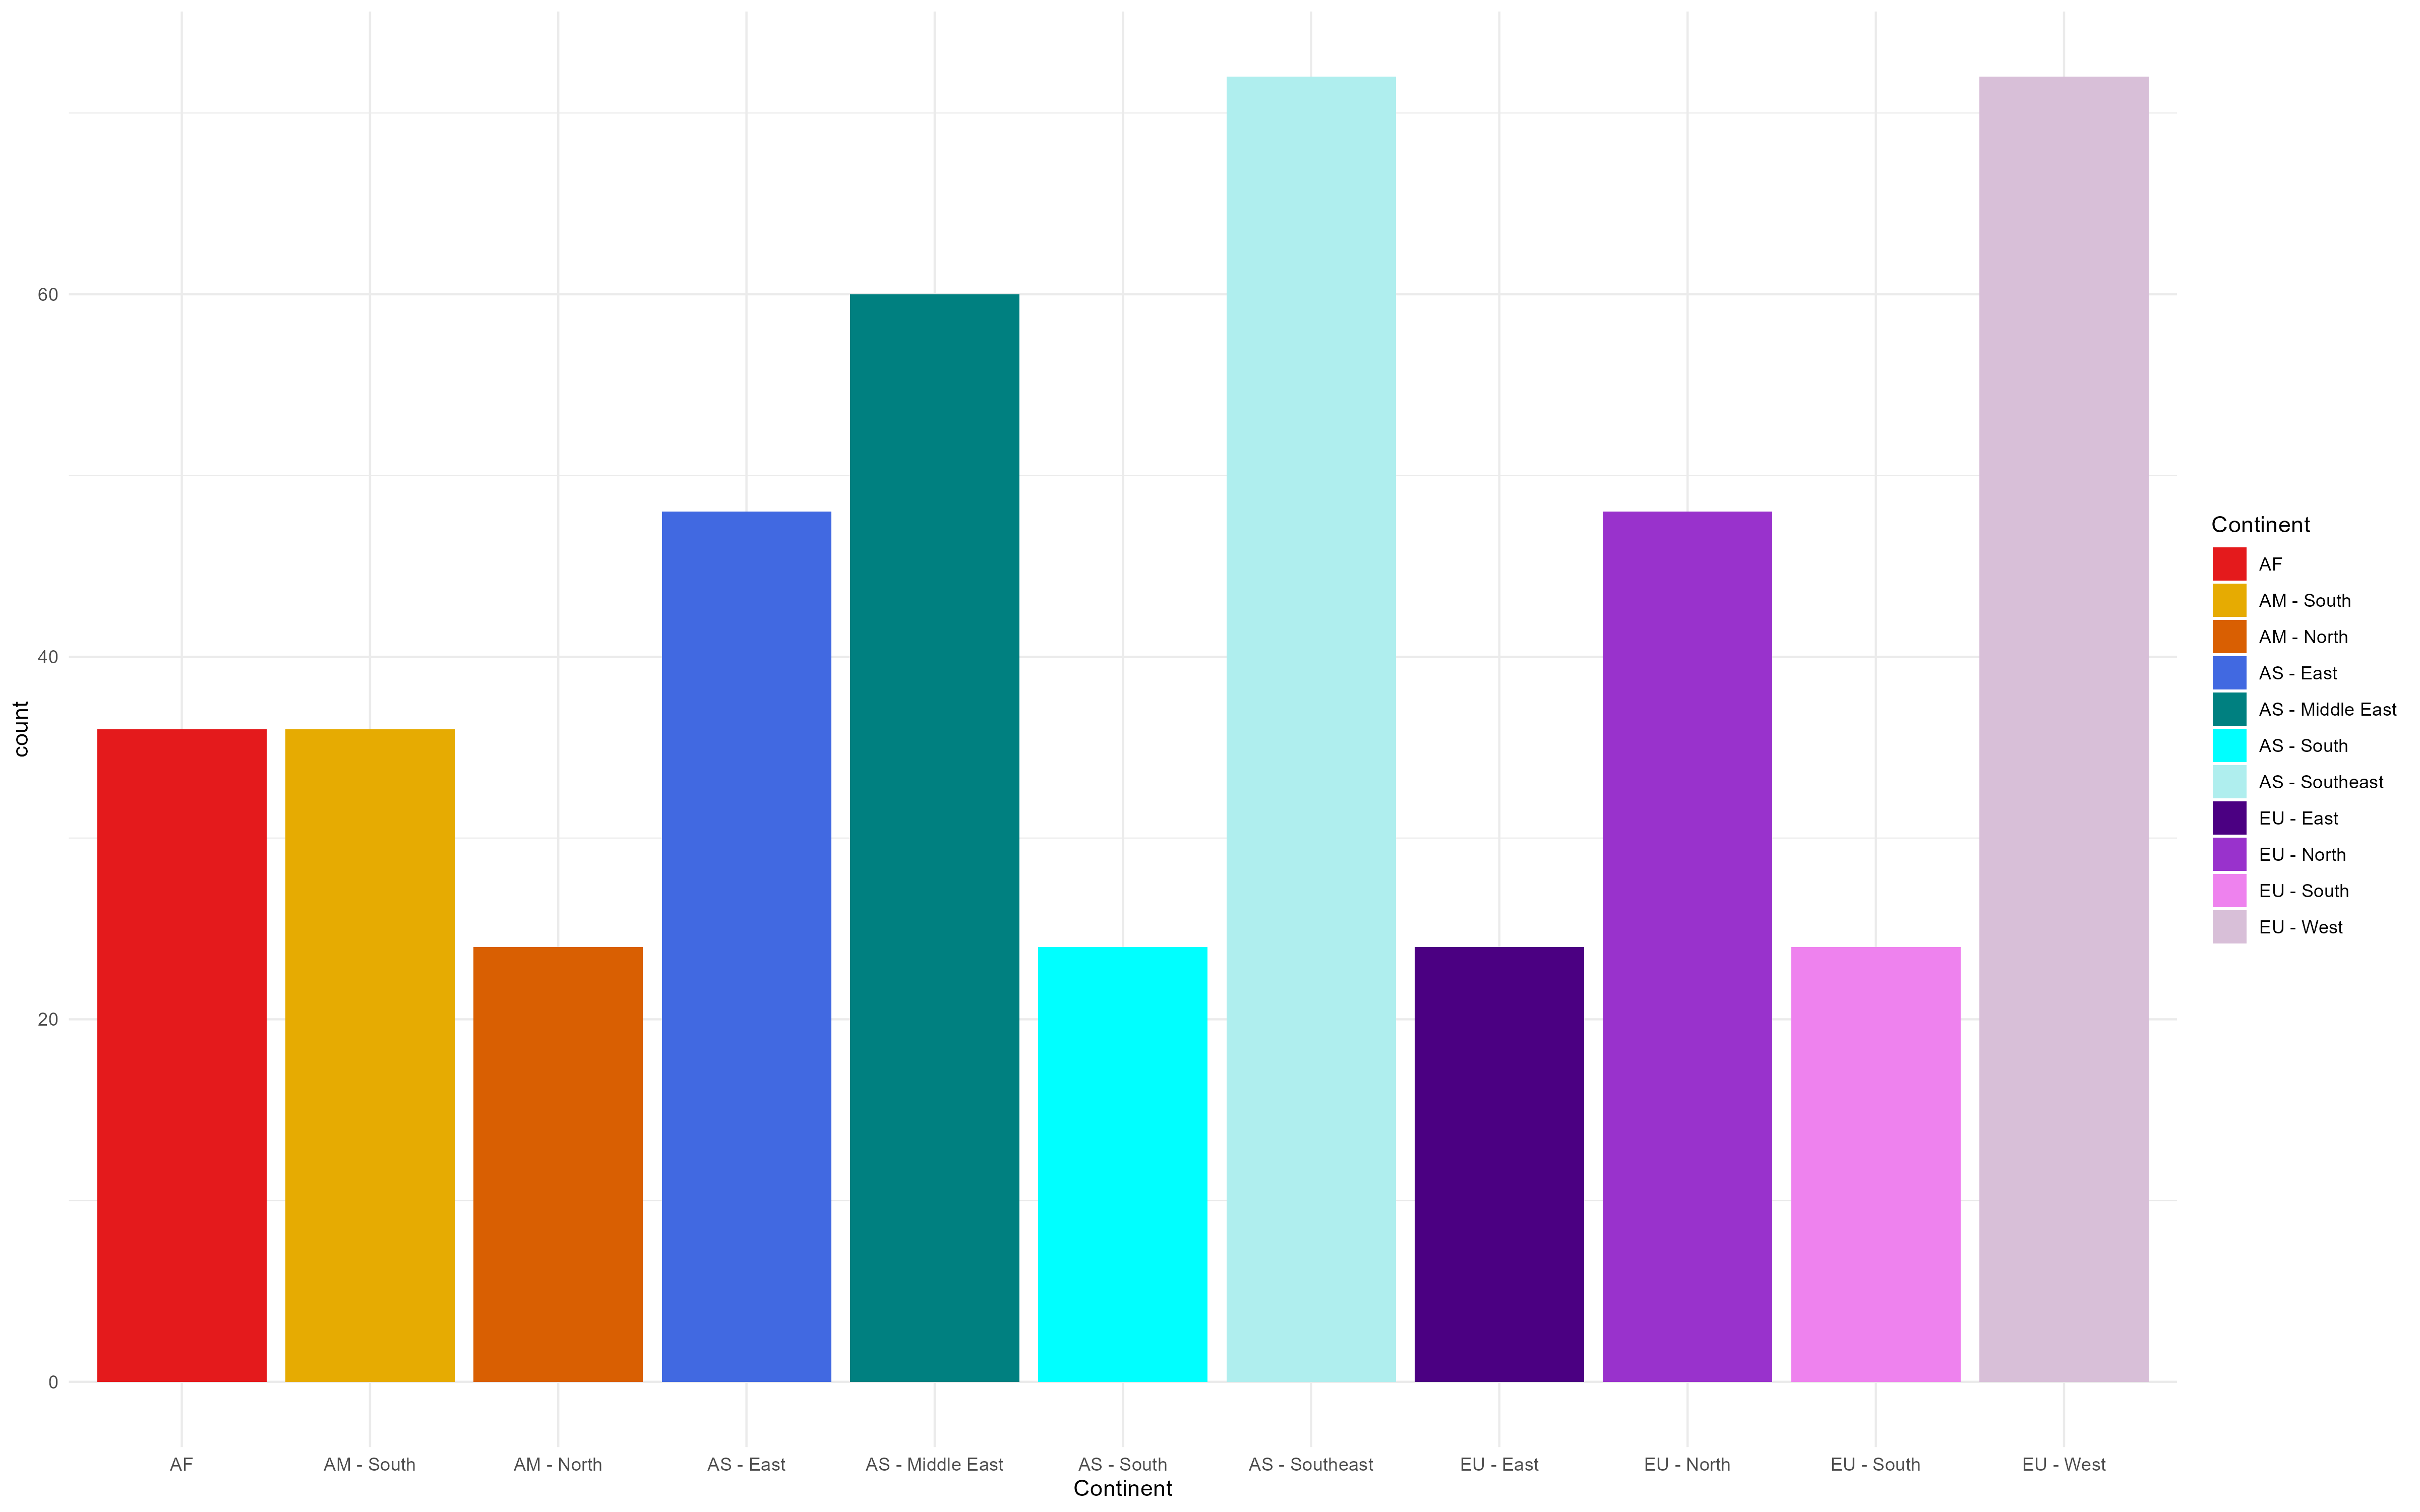
\includegraphics[width=\textwidth]{img/Colored_Correlation_Chart_Regions.png}
    \caption{Number of observations per region, extracted from (Figure \ref{fig:Correlation_Chart})}
    \label{fig:Correlation_Chart_Regions}
\end{figure}

\begin{figure}[H]
    \centering
    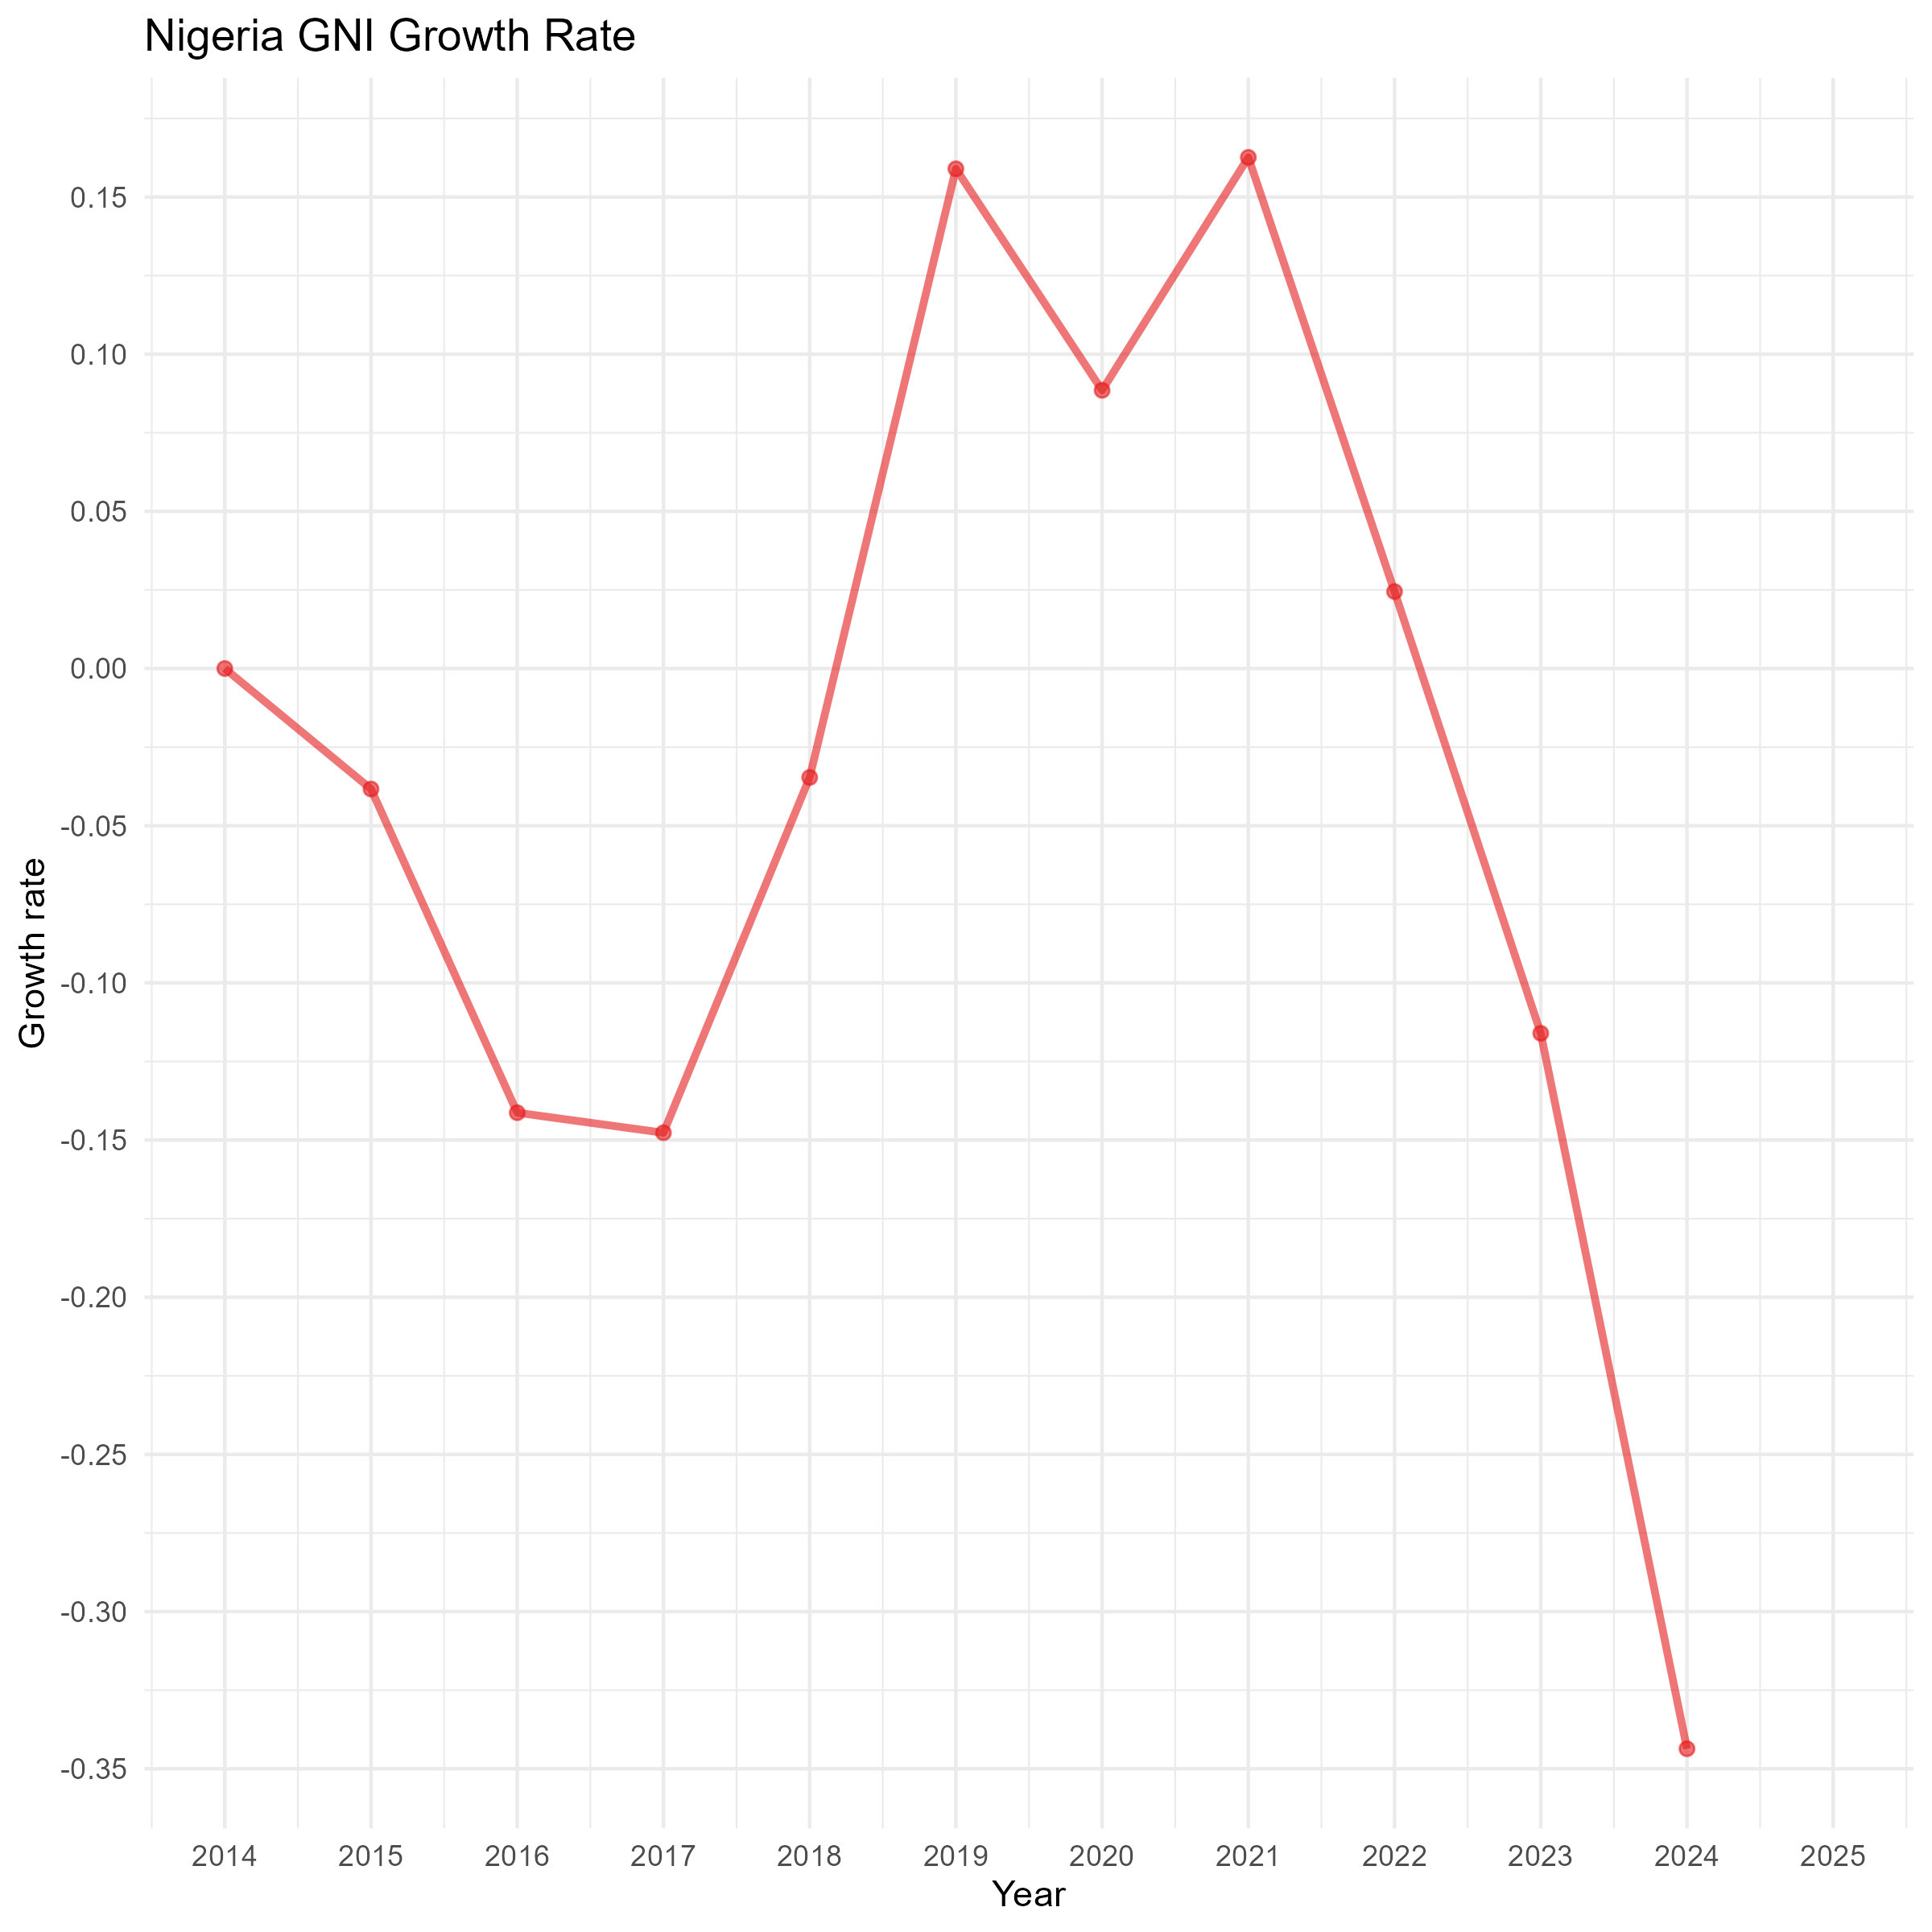
\includegraphics[width=\textwidth]{img/Nigeria_GNI_Drop.png}
    \caption{Nigeria's GNI decrease}
    \label{fig:Nigeria_GNI_Drop}
\end{figure}

\begin{figure}[H]
    \centering
    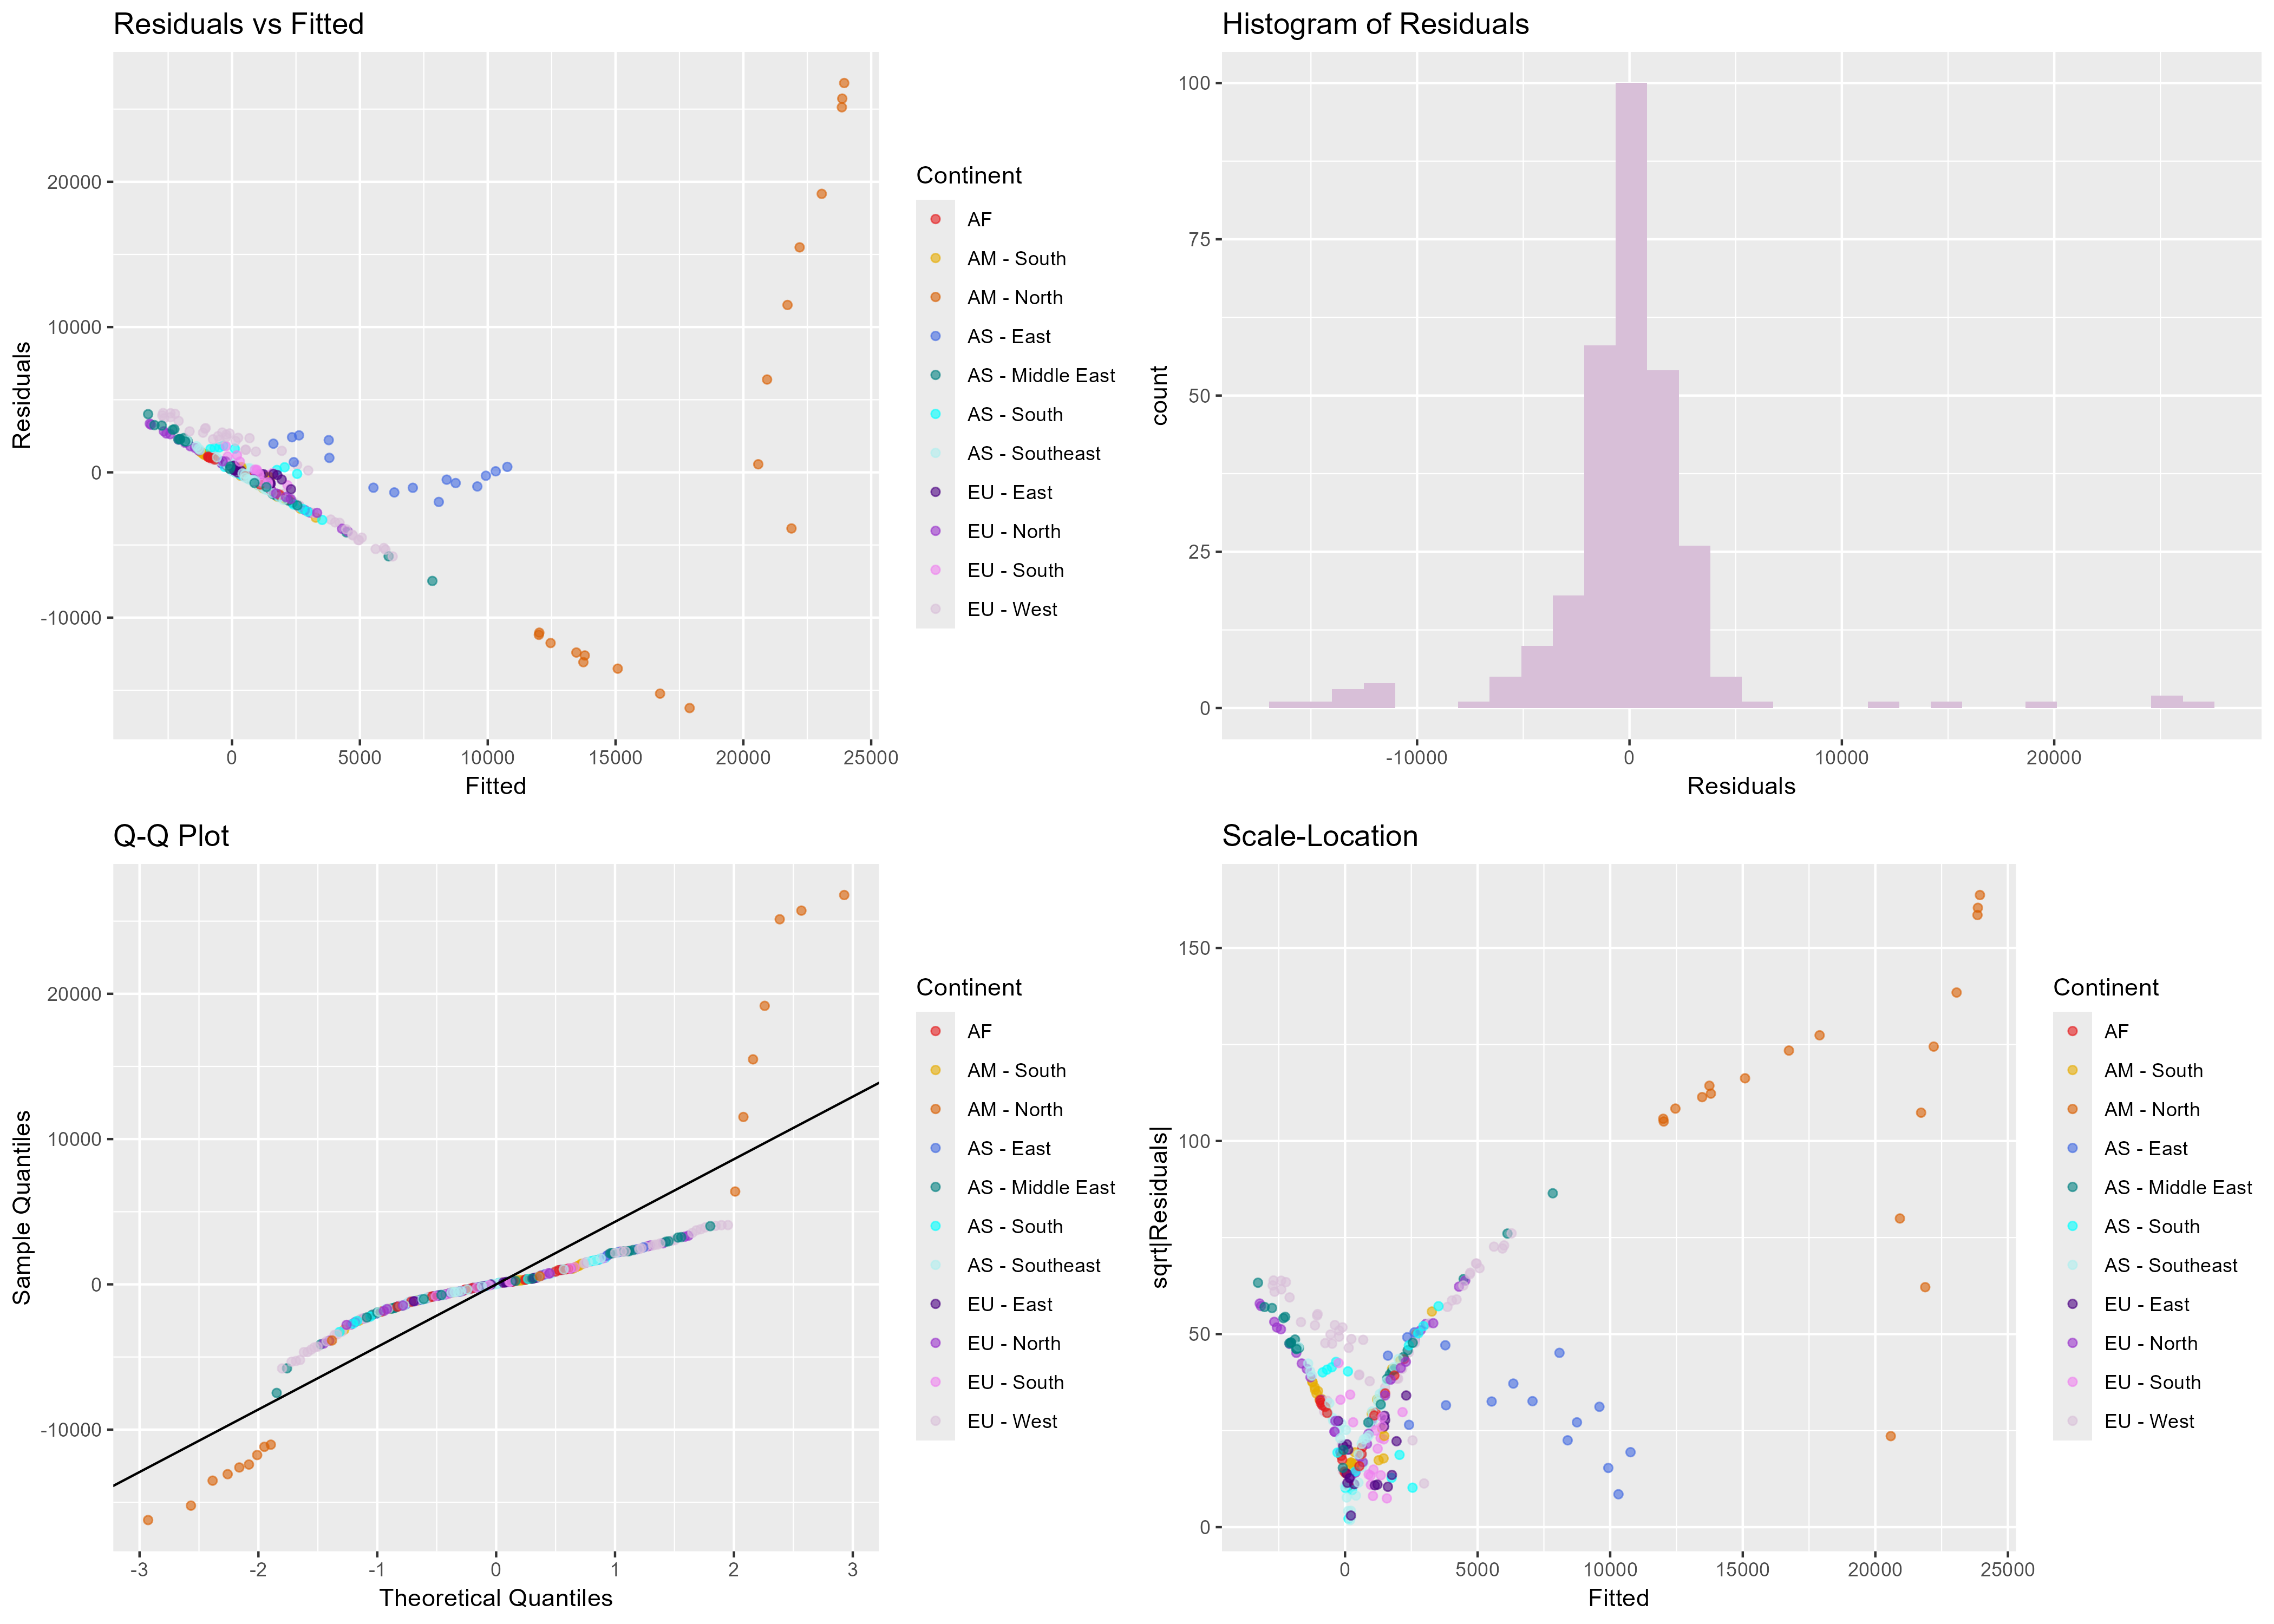
\includegraphics[width=\textwidth]{img/Non_Log_Model_Colored_Graph.png}
    \caption{Diagnostic Residual Plots for the Non-Log Model}
    \label{fig:Non_Log_Model}
\end{figure}
%*******************************************************
% FinalDedication
%*******************************************************
%\input{back/FinalDedication}

\end{document}